\documentclass[10pt,xcolor={dvipsnames}]{beamer}
\usepackage{beamerthemesplit}
\usepackage[orientation=landscape,size=custom,width=16,height=9,scale=0.4,debug]{beamerposter} 
\usepackage[utf8]{inputenc}

%%%%%import code matlab%%%%%%%%%%%%%
\usepackage{listings}
\usepackage{xsavebox} % file-size-efficient saveboxes
%\usepackage{animate}  % for animated scrolling
\usepackage{MnSymbol} % \triangle, \triangledown for scroll buttons
\usepackage{media9}   % buttons
\usepackage{xintexpr} % calculate expressions

% Code colors (Irrelevant from the presentation color theme!)
\definecolor{codemaincolor}{RGB}{0, 0, 0}
\definecolor{codebackgroundcolor}{RGB}{255, 255, 255}
\definecolor{codekeywordcolor}{RGB}{0, 0, 255}
\definecolor{codestringcolor}{RGB}{163, 21, 21}
\definecolor{codecommentcolor}{RGB}{39, 139, 39}
\definecolor{codeusertypecolor}{RGB}{43, 145, 175}

\usepackage{listings}
\usepackage{lstautogobble}
\lstset {
	basicstyle={\scriptsize \ttfamily \color{codemaincolor}},
	backgroundcolor=\color{codebackgroundcolor},
	autogobble = true,
	tabsize = 2,
	xleftmargin=0pt,
	xrightmargin=0pt,
	aboveskip=0pt, % \medskipamount,
	belowskip=0pt, % \medskipamount,
	literate={\ \ }{{\ }}1
}
% Code C++ style
\lstdefinestyle{C++} {
	language=C++,
	otherkeywords = {final, override, noexcept},
	keywordstyle = {\color{codekeywordcolor}},
	stringstyle = {\color{codestringcolor}},
	commentstyle = {\color{codecommentcolor}\em},
	% Class and types highlighting
	classoffset=1, % starting new class
	morekeywords={vector, ostream, unique_ptr, shared_ptr, T, device_t, abstract_device, device_one, device_two, device_three, executable_device, measurable_device, my_device, concept_t, model, device_one_model, device_two_model, sensor_t, history_t},
	keywordstyle=\color{codeusertypecolor},
	classoffset=0,
}


% \smoothScroll[<animate opts>]{<xsavebox id>}{<viewport height>}{<steps>}{<steps per sec>}
\newcommand{\smoothScroll}[5][]{%
	\savebox\measBox{\xusebox{#2}}%
	\edef\boxwd{\the\wd\measBox}%
	\edef\boxht{\the\ht\measBox}%
	\edef\boxtht{\the\dimexpr\ht\measBox+\dp\measBox\relax}%
	\edef\portht{\the\dimexpr#3\relax}%
	\begin{animateinline}[#1,label={#2},width=\boxwd,height=\portht]{#5}%
		\multiframe{#4}{%
			dRaiseLen=\the\dimexpr-\boxht+\portht\relax+\the\dimexpr(\boxtht-\portht)/%
			\numexpr#4-1\relax\relax
		}{%
			\begin{minipage}[b][\portht][b]{\boxwd}%
				\raisebox{\dRaiseLen}[0pt][0pt]{\xusebox{#2}}%
			\end{minipage}%
		}%
	\end{animateinline}%
}
\newsavebox\measBox % for measuring purposes

% \topScrollButton{<xsavebox id>}{<step>}
\newcommand{\topScrollButton}[2]{%
	\mediabutton[
	jsaction={
		if(event.shift){anim['#1'].pause();anim['#1'].frameNum=0;}
		else try{anim['#1'].frameNum-=#2}catch(e){anim['#1'].frameNum=0;}
	}
	]{\fboxsep=0pt\framebox[\widthof{\xusebox{#1}}][c]{%
			\tiny\strut\raisebox{-0.2\height}{$\triangle\triangle\triangle$}}%
	}%
}

% \botScrollButton{<xsavebox id>}{<step>}
\newcommand{\botScrollButton}[2]{%
	\mediabutton[
	jsaction={
		if(event.shift){anim['#1'].pause();anim['#1'].frameNum=anim['#1'].numFrames-1;}
		else try{anim['#1'].frameNum+=#2}catch(e){anim['#1'].frameNum=anim['#1'].numFrames-1;}
	}
	]{\fboxsep=0pt\framebox[\widthof{\xusebox{#1}}][c]{%
			\tiny\strut\raisebox{0.1\height}{$\triangledown\triangledown\triangledown$}}%
	}%
}

% \begin{codescroll}[<lstlisting opts>]{<xsavebox id>}{<total lines>}{<viewport lines>}
	\lstnewenvironment{codescroll}[4][style=C++]
	{\lstset{#1}\xlrbox{#2}\noindent\minipage{\linewidth}}
	{\endminipage\endxlrbox%
		\def\lnsperframe{28}% max lines without the buttons you have to change this value for different margins, beamer themes etc.
		\def\lnht{5}% height of each line
		\def\lnspersec{3}% scroll number of lines per second
		\def\htpercentage{\xintthefloatexpr #4 / \lnsperframe \relax}% calculate the height of the scroll area
		\def\steps{\xintexpr #3 - #4 + 1 \relax}% steps needed to go from the first to last line
		\def\viewportheight{\xinttheiexpr (#3 + 1)  * \lnht \relax}% total height of the viewport
		\def\btnstep{\xintthefloatexpr \viewportheight / \steps \relax}% step to in(dec)crease when press the buttons
		\def\stepspersec{\xintthefloatexpr \lnspersec * \btnstep \relax}% scroll speed
		\topScrollButton{#2}{\btnstep}\\%
		\smoothScroll{#2}{\htpercentage\textheight}{\viewportheight}{\stepspersec}\\%
		\raisebox{2ex}{\botScrollButton{#2}{\btnstep}}%
	}

\lstset{ 
	language=Matlab,                		% choose the language of the code
	%	basicstyle=10pt,       				% the size of the fonts that are used for the code
	%numbers=left,                  			% where to put the line-numbers
	%numberstyle=\footnotesize,      		% the size of the fonts that are used for the line-numbers
	%stepnumber=1,                   			% the step between two line-numbers. If it's 1 each line will be numbered
	%numbersep=5pt,                  		% how far the line-numbers are from the code
	%	backgroundcolor=\color{white},  	% choose the background color. You must add \usepackage{color}
	showspaces=false,               		% show spaces adding particular underscores
	showstringspaces=false,         		% underline spaces within strings
	showtabs=true,                 			% show tabs within strings adding particular underscores
	frame=single,	                			% adds a frame around the code
	tabsize=2,                				% sets default tabsize to 2 spaces
	%	captionpos=b,                   			% sets the caption-position to bottom
	breaklines=true,                			% sets automatic line breaking
	breakatwhitespace=false,        		% sets if automatic breaks should only happen at whitespace
	escapeinside={\%*}{*)}          		% if you want to add a comment within your code
}

%%%%%%%%%%%%%%%%%%%%%%%%%%%%%%%%%%%

%%%%%%%%%%%%%%%%%%%%%%%%%%%%%%%%%%%%%%%%%%
%ini buat bikin diagram blocks
\usepackage{tikz}
\usetikzlibrary{positioning}

%%%%%%%%%%%%%%%%%%%%%%%%%%%%%%%%%%%%%%%%%%

% Required package
\usepackage{animate}
\usepackage{movie15}				%package insert video
%\usepackage{media9,graphicx}			%video with thumbnail
\usepackage{ragged2e}
\usepackage{multirow,rotating}
\usepackage{color}
\usepackage{hyperref}
\usepackage{tikz-cd}
\usepackage{array}
\usepackage{siunitx}
%\usepackage{mathtools,nccmath}%
\usepackage{etoolbox, xparse} 
\usetheme{CambridgeUS}
\usepackage{natbib}
\usecolortheme{dolphin}

% set colors
\definecolor{myNewColorA}{RGB}{0, 0, 128} %{46, 162, 151}
\definecolor{myNewColorB}{RGB}{253, 203, 44} %{255, 235, 59}
\definecolor{myNewColorC}{RGB}{253, 203, 44} % {130,138,143}
\setbeamercolor*{palette primary}{bg=myNewColorC}
\setbeamercolor*{palette secondary}{bg=myNewColorB, fg = white}
\setbeamercolor*{palette tertiary}{bg=myNewColorA, fg = white}
\setbeamercolor*{titlelike}{fg=myNewColorA}
\setbeamercolor*{title}{bg=myNewColorA, fg = white}
\setbeamercolor*{item}{fg=myNewColorA}
\setbeamercolor*{caption name}{fg=myNewColorA}
\usefonttheme{professionalfonts}


%------------------------------------------------------------
% \titlegraphic{\includegraphics[height=0.75cm]{ua_eng_logo.png}} 

% logo of my university

\titlegraphic{

\includegraphics[height=1.5cm]{Lambang dan logo UGM/Logo Horizontal Stack-Up.png}
	
}

\setbeamerfont{title}{size=\large}
\setbeamerfont{subtitle}{size=\small}
\setbeamerfont{author}{size=\small}
\setbeamerfont{date}{size=\footnotesize}
\setbeamerfont{institute}{size=\footnotesize}
\title[UGM]{Kendali Kecepatan dan Posisi Motor DC}%title
%\subtitle{ }%%subtitle
\author[Kelompok 1]{Priyova M. Rafief\inst{1}, Karunia Dini F.\inst{1}, Octsana Dhiyaa W.\inst{1}, Bodhi Setiawan\inst{1}}%%authors

\institute[UGM]{Universitas Gadjah Mada\inst{1}}
\date[\textcolor{white}{PSKL, 2022}]
{Praktikum Sistem Kendali Lanjut}

%------------------------------------------------------------
%This block of commands puts the table of contents at the 
%beginning of each section and highlights the current section:
%\AtBeginSection[]
%{
	%  \begin{frame}
		%    \frametitle{Contents}
		%    \tableofcontents[currentsection]
		%  \end{frame}
	%}

\AtBeginSection[]{
	\begin{frame}
		\vfill
		\centering
		\begin{beamercolorbox}[sep=8pt,center,shadow=true,rounded=true]{title}
			\usebeamerfont{title}\insertsectionhead\par%
		\end{beamercolorbox}
		\vfill
	\end{frame}
}
% ------Contents below------
%------------------------------------------------------------

\begin{document}
	
	%The next statement creates the title page.

	\frame{\titlepage}
	
	\begin{frame}
		\frametitle{Anggota Kelompok 1}
		\begin{enumerate}
			\item Priyoya M. Rafief (20/457197/SV/17644)
			\item Karunia Dini F. (20/464248/SV/18567)
			\item Octsana Dhiyaa W. (20/464253/SV/18572)
			\item Bodhi Setiawan (20/464239/SV/18558)
		\end{enumerate}
	\end{frame}
	
	\begin{frame}
		\frametitle{Isi Pembahasan}
		    \tableofcontents
	\end{frame}
	
	\section{Gambaran Umum Proyek Sistem Kendali Motor DC}
	
	\begin{frame}{Diagram Sistem}
		\centering
		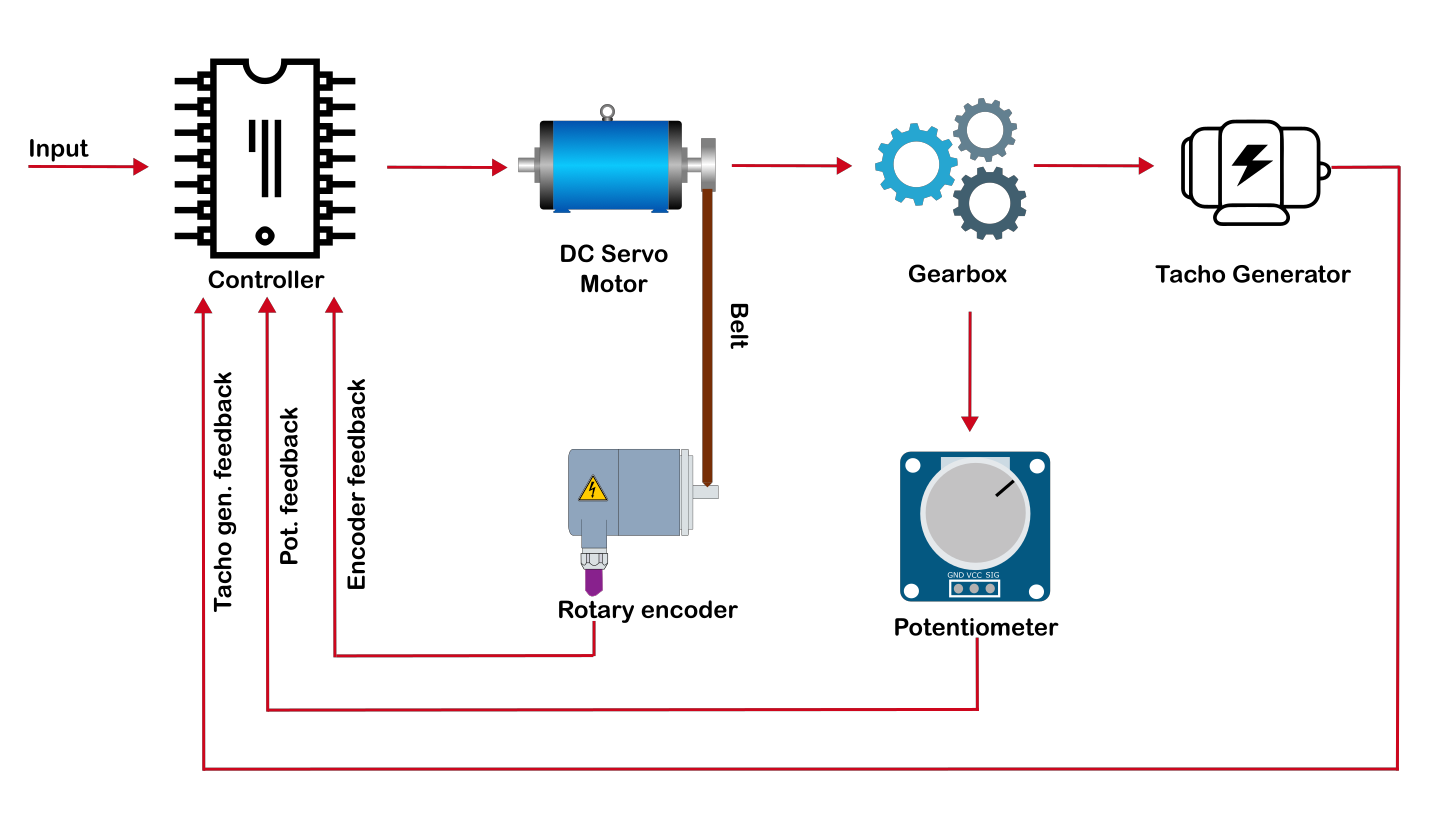
\includegraphics[width=10cm]{Gambar Lain/diagramDCservo.png}
	\end{frame}

	\begin{frame}{Flowchart Kerja Program Pada Alat}
		\centering
		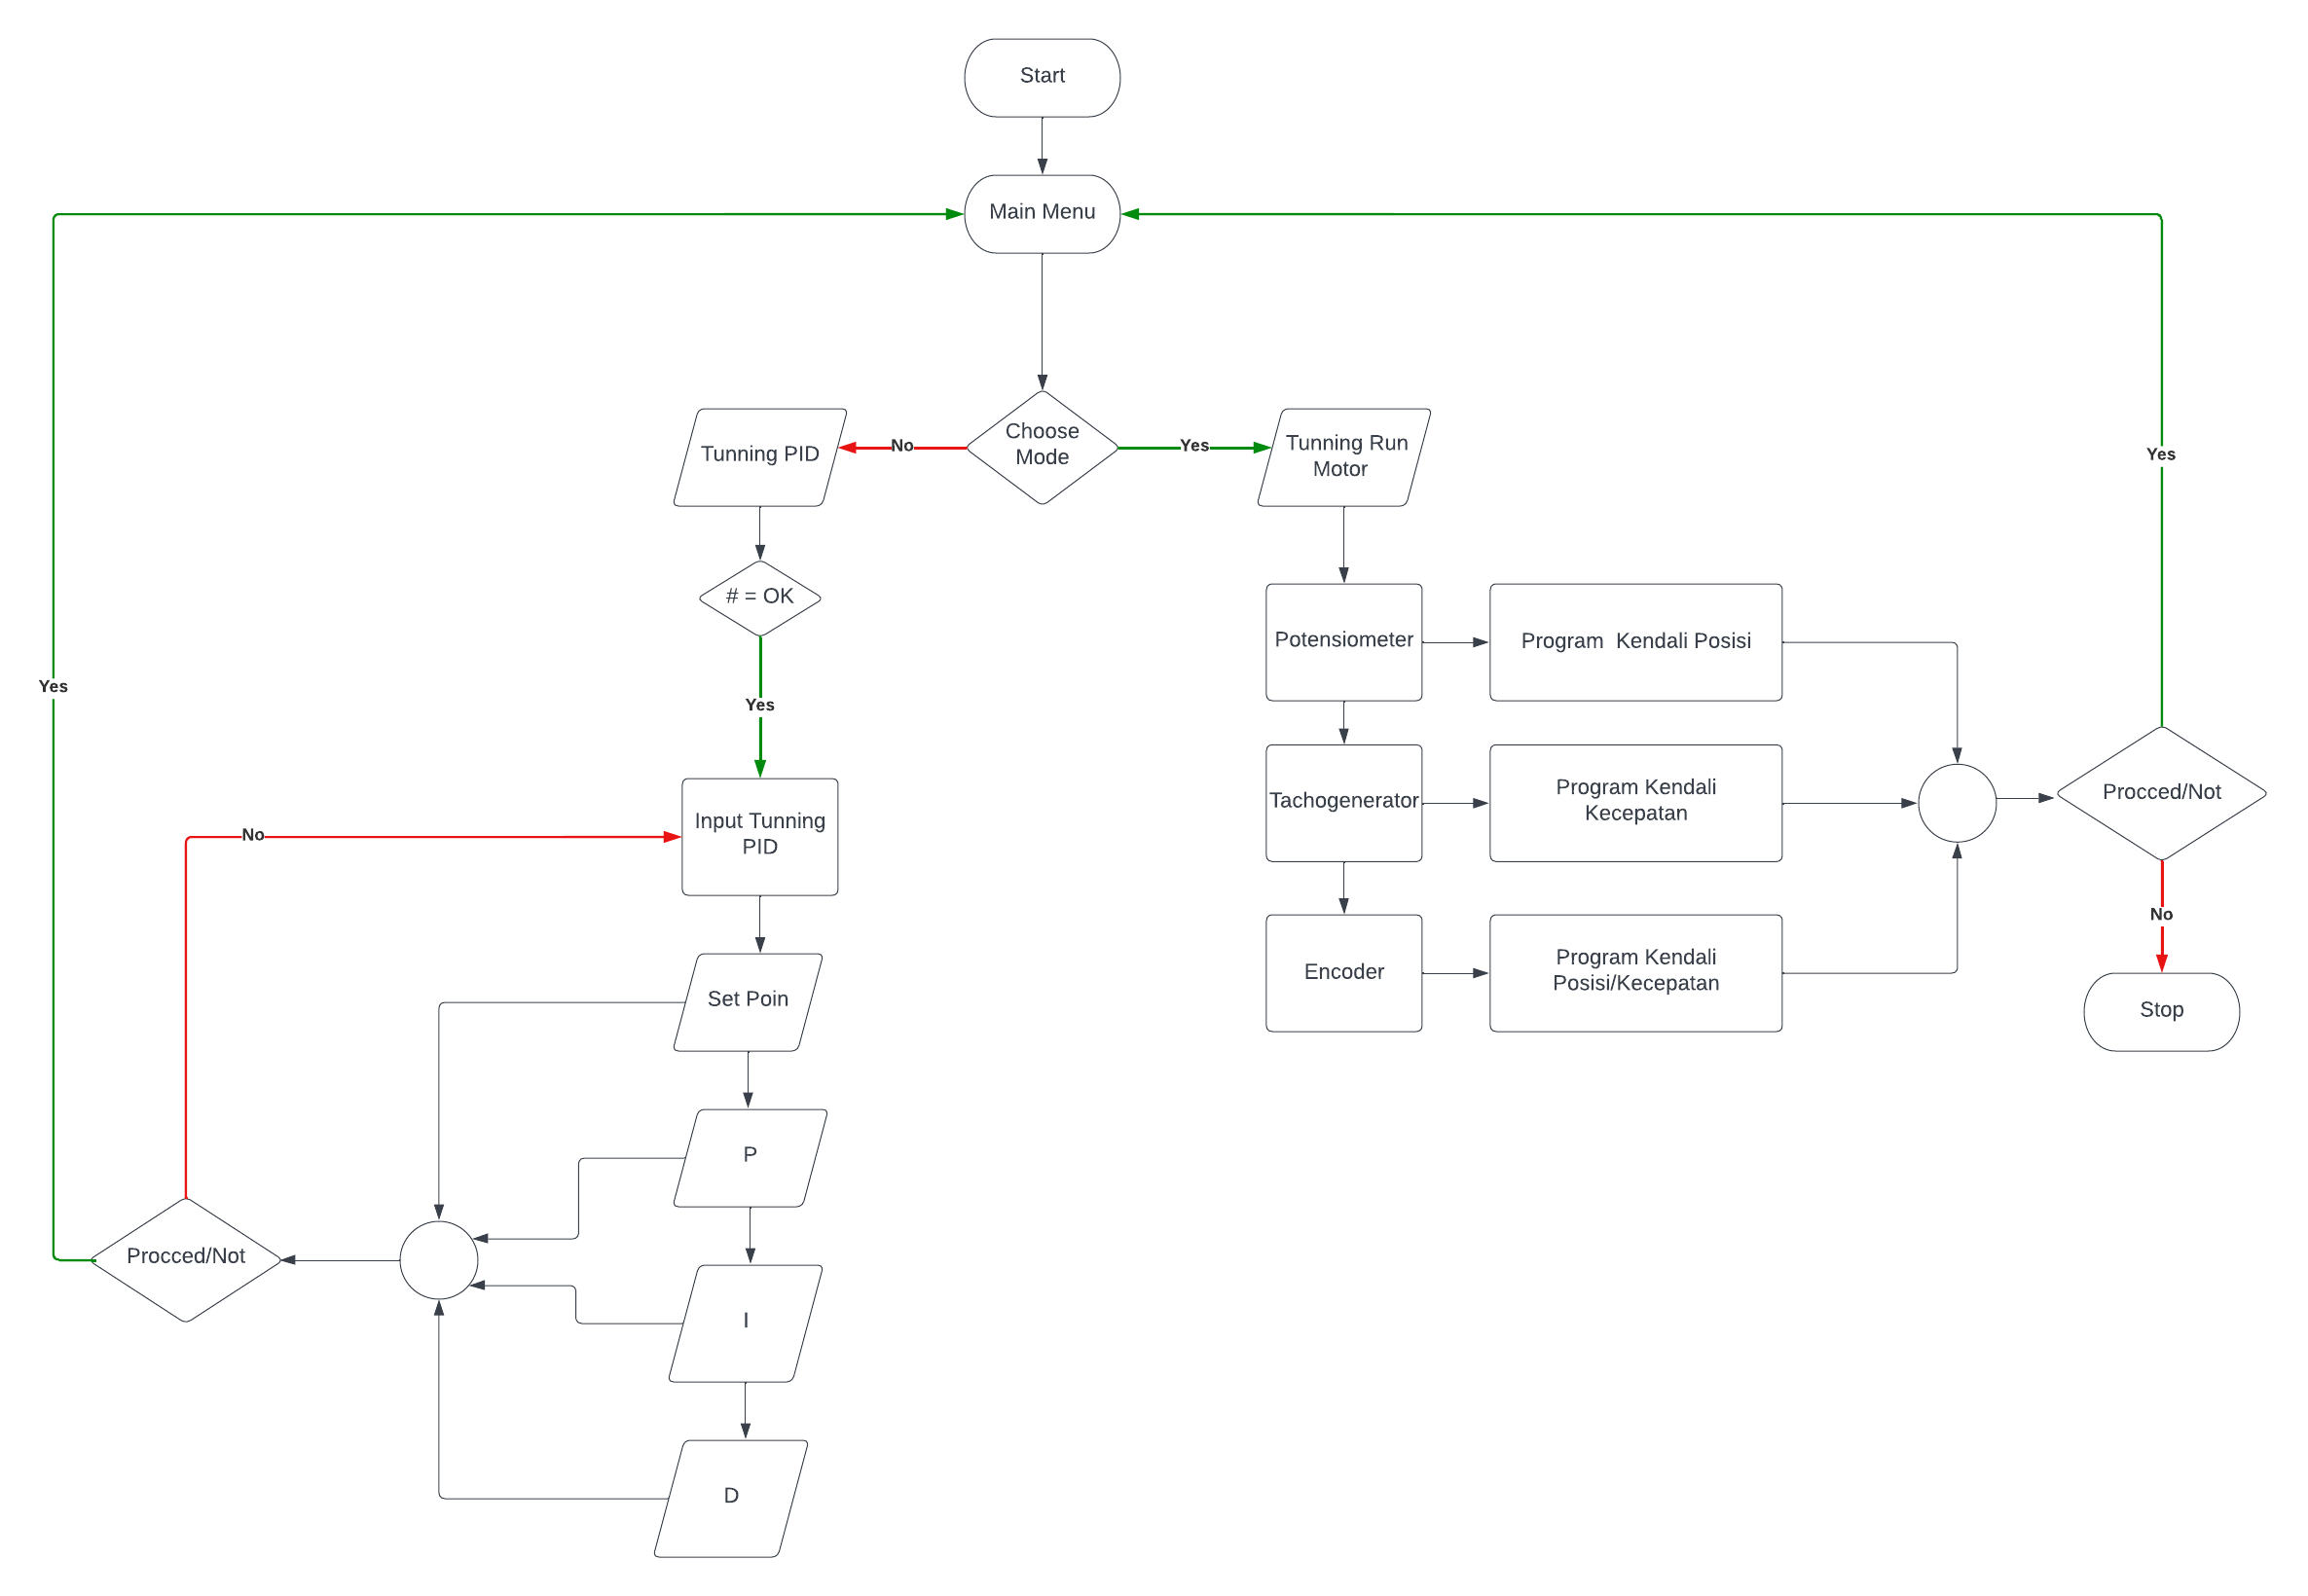
\includegraphics[width=10cm]{Gambar Lain/Flowchart Sistem.png}
	\end{frame}
	
	\section{Pemodelan Sistem Motor DC}
	
	\begin{frame}{Pengertian Motor DC}
		\begin{columns}[T]% align columns
			\begin{column}{0.48\textwidth}
				\color{black}\rule{\linewidth}{4pt}
				
					Motor DC atau dalam bahasa Indonesia disebut motor arus searah adalah jenis motor listrik yang mengubah energi listrik arus searah menjadi energi mekanis. Bentuk energi yang dihasilkan berupa putaran. Prinsip kerja motor aru searah berdasarkan pada interaksi antara dua fluks magnetik yang disebut dengan kumparan medan dan kumparan jangkar. Kumparan medan menghasilkan fluks magnet dengan arah dari kutub utara ke kutub selatan, sedangkan kumparan jangkar menghasilkan fluks magnetik yang melingkar. \newline \textit{Sumber: Wikipedia}		
			\end{column}%
			\hfill%
			\begin{column}{0.48\textwidth}
				\color{myNewColorA}\rule{\linewidth}{4pt}
				Ilustrasi Motor DC:\newline
				\animategraphics[loop,width=7cm]{10}{Gambar Lain/PMDC/PMDC-}{0}{3}
			\end{column}
		\end{columns}
	\end{frame}
	\begin{frame}{Struktur Fisik}
		\begin{columns}[T] % align columns
			\begin{column}{0.48\textwidth}
				Parameter:
				\color{black}\rule{\linewidth}{4pt}
					\begin{flushleft}
					\begin{tabular}{lll}
						$J$ &:& Momen inersia rotor $(Kg.m^2)$\\
						$b$ &:& Koefisien gaya gesek viskos $(N.m.s)$\\
						$Ke$ &:& Koefisien gaya elektromotif $(V/rad/sec)$\\
						$Kt$ &:& Koefisien torsi motor $(N.m/Amp)$\\
						$R$ &:& Resistansi kumparan $(Ohm)$\\
						$L$ &:& Induktansi kumparan $(H)$\\
					\end{tabular}
				\end{flushleft}
			\end{column}%
			\hfill%
			\begin{column}{0.48\textwidth}
				Struktur:\newline
				\color{myNewColorA}\rule{\linewidth}{4pt}
				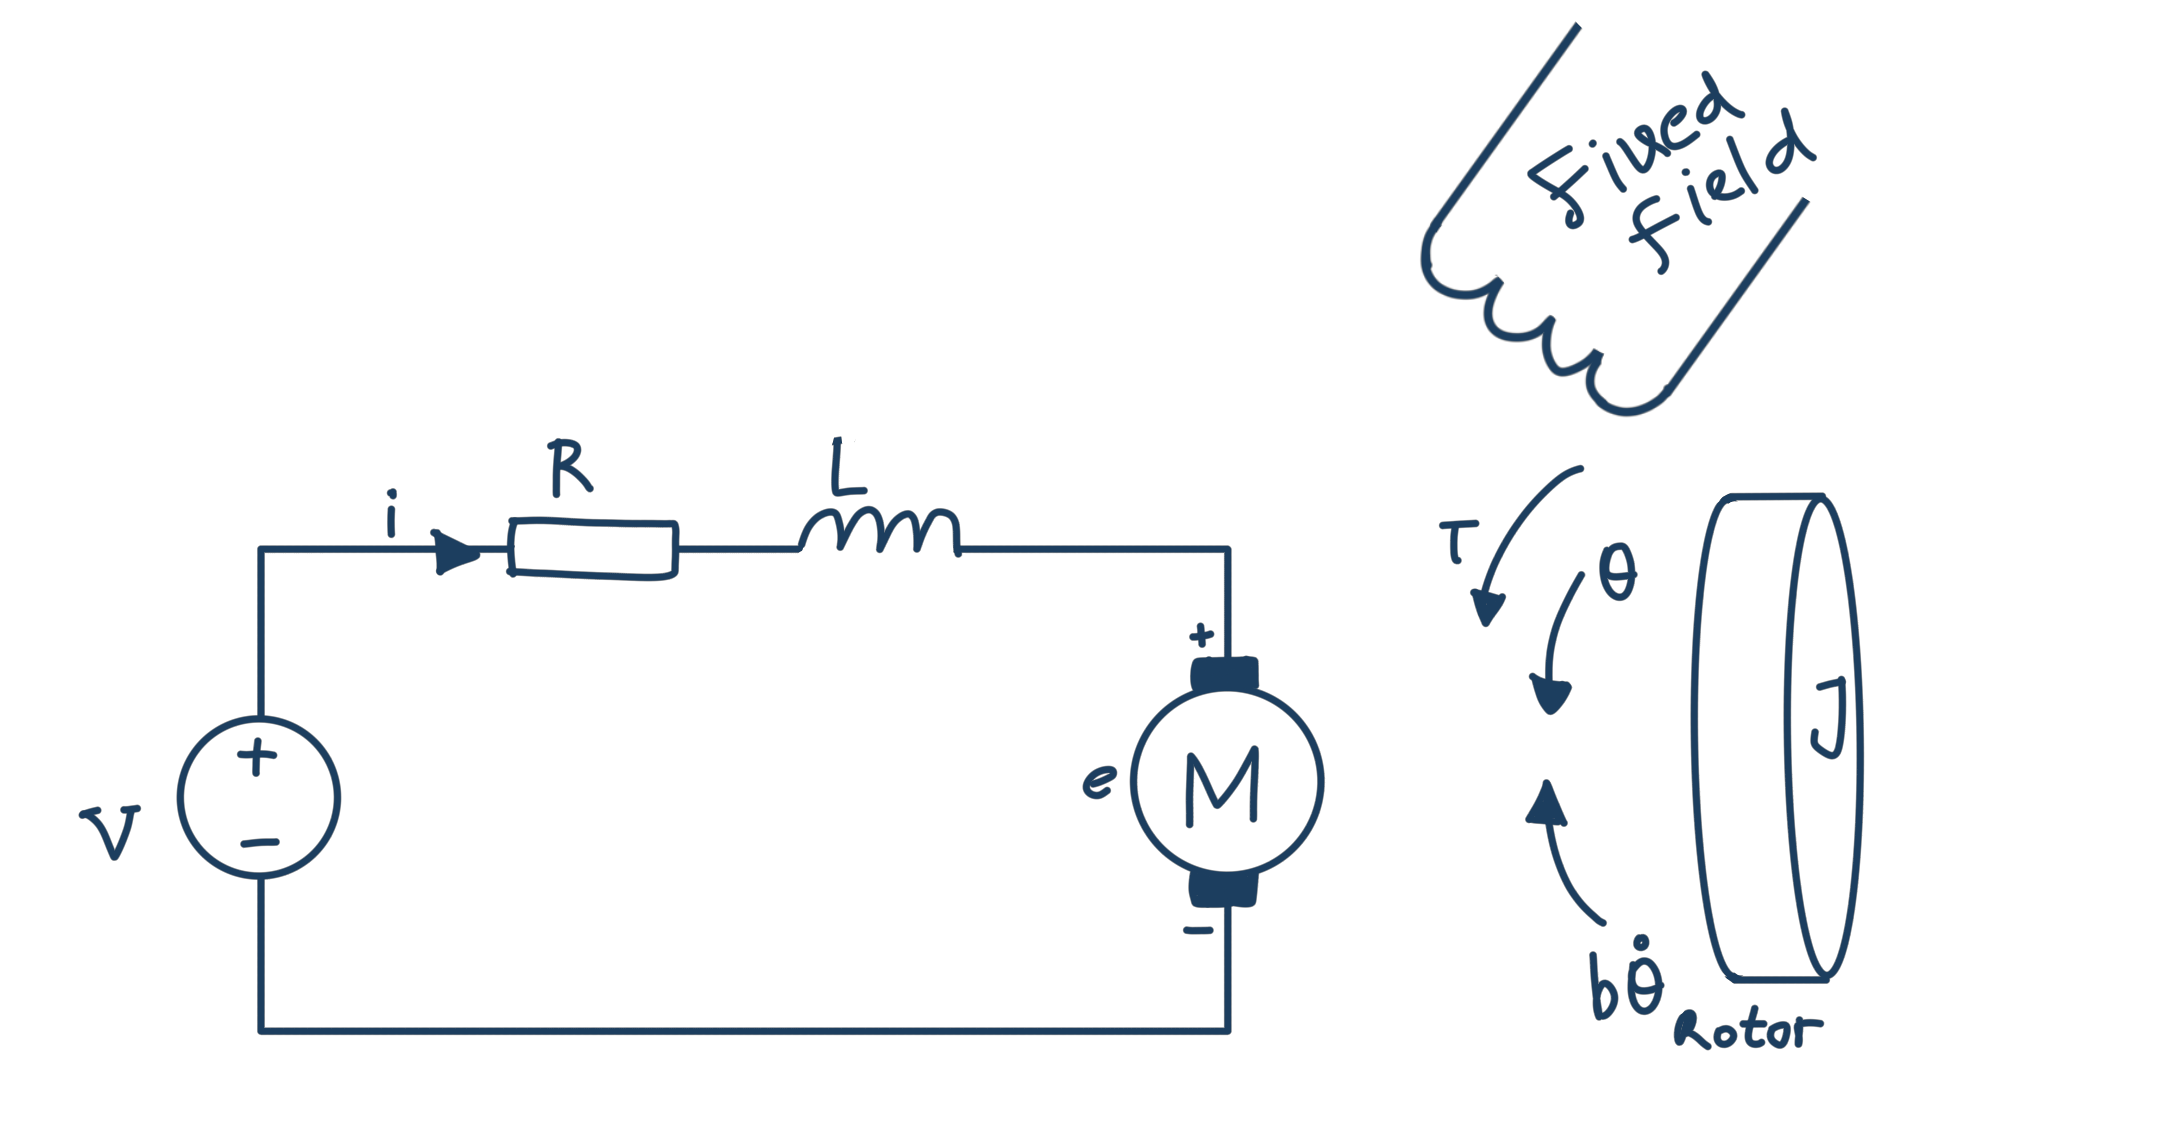
\includegraphics[width=7.5cm]{Gambar Lain/Struktur.png}
			\end{column}
		\end{columns}
\end{frame}
\begin{frame}{Diagram Blok Plant Motor DC}
	Struktur motor DC dengan parameter-parameter sebelumnya memiliki diagram blok sebagai berikut:\newline
	\begin{center}
			\begin{tikzpicture}
			% Sum shape
			\node[draw, circle, minimum size=0.6cm, fill=Rhodamine!50] (sum) at (0,0){};
			
			\draw (sum.north east) -- (sum.south west)
			(sum.north west) -- (sum.south east);
			
			\draw (sum.north east) -- (sum.south west)
			(sum.north west) -- (sum.south east);
			
			\node[left=-1pt] at (sum.center){\tiny $+$};
			\node[below] at (sum.center){\tiny $-$};
			
			% Controller
			\node [draw, fill=Goldenrod, minimum width=2cm, minimum height=1.2cm, right=1cm of sum] (controller) {\large $\frac{1}{Ls+R}$};
			
			\node [draw, minimum width=1cm, minimum height=0.6cm, below=0.3cm of controller] (text1) {\textit{Electrical}};
			
			% System H(s)
			\node [draw, fill=SpringGreen, minimum width=1cm, minimum height=1cm, right=1.5cm of controller] (system1) {$Kt$};
			
			\node [draw, fill=Aquamarine, minimum width=2cm, minimum height=1.2cm, right=4cm of controller] (system2) {\large $\frac{1}{Js+b}$};
			
			\node [draw, minimum width=1cm, minimum height=0.6cm, below=0.3cm of system2] (text2) {\textit{Mechanical}};
			
			% Sensor block
			\node [draw, fill=SeaGreen, minimum width=1cm, minimum height=1cm,  below right= 1.5cm and 1.5cm of controller]  (sensor) {$Ke$};
			
			% Arrows with text label
			\draw[-stealth] (sum.east) -- (controller.west);
			
			\draw[-stealth] (controller.east) -- (system1.west) 
			node[midway,above]{$I(s)$};
			
			\draw[-stealth] (system1.east) -- (system2.west) 
			node[midway,above]{$T(s)$};
			
			\draw[-stealth] (system2.east) -- ++ (1.25,0) 
			node[midway](output){}node[midway,above]{$\dot{\theta}(s)$};
			
			\draw[-stealth] (output.center) |- (sensor.east);
			
			\draw[-stealth] (sensor.west) -| (sum.south) 
			node[very near start,above]{$e(s)$};
			
			\draw (sum.west) -- ++(-1,0) 
			node[midway,above]{$V(s)$};
		\end{tikzpicture}
	\end{center}
\end{frame}

\begin{frame}{Fungsi Alih}
	Diagram blok \textit{plant} motor DC menghasilkan persamaan fungsi alih berikut:
	\begin{equation}
		\frac{\dot{\theta}(s)}{V(s)}=\frac{Kt}{(Js+b)(Ls+R)+KtKe} \qquad \left[\frac{rad/sec}{V}\right] 
	\end{equation} 
	Persamaan di atas merupakan fungsi alih kecepatan motor DC. Dengan mengintegralkan fungsi alih tersebut, maka diperoleh fungsi alih untuk posisi motor DC:
	\begin{equation}
		\frac{\theta(s)}{V(s)}=\frac{Kt}{s((Js+b)(Ls+R)+KtKe)} \qquad \left[\frac{rad}{V}\right]
		\label{position}
	\end{equation}
\end{frame}

\begin{frame}{\textit{State Space}}
	\begin{columns}[T]
		\begin{column}{0.5\textwidth}
			Kecepatan:
			\color{black}\rule{\linewidth}{4pt}
			\begin{equation}
				\begin{split}
					\frac{\delta}{\delta t}
					\begin{bmatrix}
						\dot{\theta} \\ i
					\end{bmatrix}
					=
					\begin{bmatrix}
						-\frac{b}{J} & \frac{Kt}{J}\\
						-\frac{Ke}{L} & -\frac{R}{L}
					\end{bmatrix}
					\begin{bmatrix}
						\dot{\theta} \\ i
					\end{bmatrix}
					+
					\begin{bmatrix}
						0 \\ \frac{1}{L}
					\end{bmatrix}
					V\\
					y=
					\begin{bmatrix}
						1 & 0
					\end{bmatrix}
						\begin{bmatrix}
						\dot{\theta} \\ i
					\end{bmatrix}
				\end{split}
			\end{equation}
		\end{column}%
		\hfill%
		\begin{column}{0.5\textwidth}
			Struktur:\newline
			\color{myNewColorA}\rule{\linewidth}{4pt}
			\begin{equation}
				\begin{split}
					\frac{\delta}{\delta t}
					\begin{bmatrix}
						\theta \\ \dot{\theta} \\ i
					\end{bmatrix}
					=
					\begin{bmatrix}
						0 & 1 & 0\\
						0 & -\frac{b}{J} & \frac{Kt}{J}\\
						0 & -\frac{Ke}{L} & -\frac{R}{L}
					\end{bmatrix}
					\begin{bmatrix}
						\theta \\ \dot{\theta} \\ i
					\end{bmatrix}
					+
					\begin{bmatrix}
						0 \\ 0 \\ \frac{1}{L}
					\end{bmatrix}
					V\\
					y=
					\begin{bmatrix}
						1 & 0 & 0
					\end{bmatrix}
					\begin{bmatrix}
						\theta \\ \dot{\theta} \\ i
					\end{bmatrix}
				\end{split}
			\end{equation}
		\end{column}
	\end{columns}
\end{frame}

\section{Perancangan Kendali PID Motor DC}
\begin{frame}{Apa Itu Kendali PID?}
	\begin{itemize}
		\item PID=\textbf{Proportional-Integral-Derivative}
		\item Kendali mekanisme umpan balik yang biasanya dipakai pada sistem kontrol industri
		\item Secara kontinu menghitung nilai kesalahan sebagai beda antara setpoint yang diinginkan dan variabel proses terukur.
		Persamaan:
		\begin{equation}
			u(t)=K_{p}e(t)+K_{i}\int_{0}^{t}e(t)dt+K_{d}\frac{de(t)}{dt}
		\end{equation}
	\end{itemize}
\end{frame}

\begin{frame}{Mengapa Kendali PID?}
	Kendali PID berfungsi untuk meminimalkan nilai kesalahan (\textit{error}) setiap waktu dengan penyetelan variabel kontrol, seperti posisi, kecepatan, damper, daya, dan lain sebagainya.\newline
	Contoh perbandingan sistem dengan dan tanpa PID:
	\begin{center}
		\animategraphics[loop,width=7cm]{20}{Gambar Lain/posComp/posComp-}{0}{37}
	\end{center}
\end{frame}

\begin{frame}{Diagram Blok Kendali}
	\begin{center}
		\begin{tikzpicture}
			
			% Sum shape
			\node[draw, circle, minimum size=0.6cm, fill=Rhodamine!50] (sum) at (0,0){};
			
			\draw (sum.north east) -- (sum.south west)
			(sum.north west) -- (sum.south east);
			
			\draw (sum.north east) -- (sum.south west)
			(sum.north west) -- (sum.south east);
			
			\node[left=-1pt] at (sum.center){\tiny $+$};
			\node[below] at (sum.center){\tiny $-$};
			
			% Controller
			\node [draw, fill=Goldenrod, minimum width=2cm, minimum height=1.2cm, right=1cm of sum] (controller) {$C(s)$};
			
			% System H(s)
			\node [draw, fill=SpringGreen, minimum width=2cm, minimum height=1.2cm, right=1.5cm of controller] (system) {$P(s)$};
			
			% Arrows with text label
			\draw[-stealth] (sum.east) -- (controller.west)
			node[midway,above]{$e$};
			
			\draw[-stealth] (controller.east) -- (system.west) 
			node[midway,above]{$u$};
			
			\draw[-stealth] (system.east) -- ++ (1.25,0) 
			node[midway](output){}node[midway,above]{$y$};
			\draw [-stealth] (output.center) -- ++ (0,-2) -| (sum.south);
			
			\draw (sum.west) -- ++(-1,0) 
			node[midway,above]{$r$};
			
		\end{tikzpicture}
	\end{center}
	\textbf{Keterangan:}\newline
	\begin{tabular}{lll}
		$C(s)$ &:& \textit{Controller}\\
		$P(s)$ &:& \textit{Plant}\\
		$r(s)$ &:& \textit{Output} yang diinginkan\\
		$e(s)$ &:& Nilai \textit{error}\\
		$u(s)$ &:& Sinyal kendali\\
		$y(s)$ &:& \textit{Output} sesungguhnya\\
	\end{tabular}
	\end{frame}
\begin{frame}{Diagram Blok Kendali PID Motor DC: Kecepatan}
	\begin{center}
		\begin{tikzpicture}
			
			% Sum shape
			\node[draw, circle, minimum size=0.6cm, fill=Rhodamine!50] (sum) at (0,0){};
			
			\draw (sum.north east) -- (sum.south west)
			(sum.north west) -- (sum.south east);
			
			\draw (sum.north east) -- (sum.south west)
			(sum.north west) -- (sum.south east);
			
			\node[left=-1pt] at (sum.center){\tiny $+$};
			\node[below] at (sum.center){\tiny $-$};
			
			\node [draw, minimum width=1cm, minimum height=0.6cm, above right=0.3cm and -1.2cm of controller] (text2) {\textit{PID}};
			% Controller
			\node [draw, fill=Magenta, minimum width=2cm, minimum height=1.2cm, right=1cm of sum]  (controller) {$Kp+\frac{Ki}{s}+Kds$};
			
			\node [draw, minimum width=1cm, minimum height=0.6cm, above right=0.3cm and -1.5cm of system] (text2) {\textit{DC Motor}};
			% System H(s)
			\node [draw, fill=Peach, minimum width=2cm, minimum height=1.2cm, right=0.8cm of controller] (system) {$\frac{Kt}{(Js+b)(Ls+R)+KtKe}$};
			
			% Arrows with text label
			\draw[-stealth] (sum.east) -- (controller.west)
			node[midway,above]{$e(s)$};
			
			\draw[-stealth] (controller.east) -- (system.west) 
			node[midway,above]{$u(s)$};
			
			\draw[-stealth] (system.east) -- ++ (1.25,0) 
			node[midway](output){}node[midway,above]{$\dot{\theta}$};
			\draw [-stealth] (output.center) -- ++ (0,-1.5) -| (sum.south);
			
			\draw (sum.west) -- ++(-1,0) 
			node[midway,above]{$V(s)$};
		\end{tikzpicture}
	\end{center}
\end{frame}

\begin{frame}{Diagram Blok Kendali PID Motor DC: Posisi}
	\begin{center}
		\begin{tikzpicture}
			
			% Sum shape
			\node[draw, circle, minimum size=0.6cm, fill=Rhodamine!50] (sum) at (0,0){};
			
			\draw (sum.north east) -- (sum.south west)
			(sum.north west) -- (sum.south east);
			
			\draw (sum.north east) -- (sum.south west)
			(sum.north west) -- (sum.south east);
			
			\node[left=-1pt] at (sum.center){\tiny $+$};
			\node[below] at (sum.center){\tiny $-$};
			
			\node [draw, minimum width=1cm, minimum height=0.6cm, above right=0.3cm and -2cm of controller] (text2) {\textit{PID}};
			% Controller
			\node [draw, fill=Aquamarine, minimum width=2cm, minimum height=1.2cm, right=1cm of sum]  (controller) {$Kp+\frac{Ki}{s}+Kds$};
			
			\node [draw, minimum width=1cm, minimum height=0.6cm, above right=0.3cm and -2.5cm of system] (text2) {\textit{DC Motor}};
			% System H(s)
			\node [draw, fill=SkyBlue, minimum width=2cm, minimum height=1.2cm, right=0.8cm of controller] (system) {$\frac{Kt}{s((Js+b)(Ls+R)+KtKe)}$};
			
			% Arrows with text label
			\draw[-stealth] (sum.east) -- (controller.west)
			node[midway,above]{$e(s)$};
			
			\draw[-stealth] (controller.east) -- (system.west) 
			node[midway,above]{$u(s)$};
			
			\draw[-stealth] (system.east) -- ++ (1.25,0) 
			node[midway](output){}node[midway,above]{$\theta$};
			\draw [-stealth] (output.center) -- ++ (0,-1.5) -| (sum.south);
			
			\draw (sum.west) -- ++(-1,0) 
			node[midway,above]{$V(s)$};
		\end{tikzpicture}
	\end{center}
\end{frame}

\section{Simulasi Kendali PID}

\begin{frame}{Uji Perbandingan Sistem \textit{Open-loop} dengan \textit{Closed-loop} Motor DC}
	\begin{columns}[T] % align columns
		\begin{column}{0.48\textwidth}
			Program \textit{Open-loop}:
			\color{black}\rule{\linewidth}{4pt}
			\lstinputlisting[language=Matlab]{Matlab/olDCmotor.m}
		\end{column}%
		\hfill%
		\begin{column}{.48\textwidth}
			Program \textit{Closed-loop}:
			\color{blue}\rule{\linewidth}{4pt}
			\begin{center}
				\lstinputlisting[language=Matlab]{Matlab/clDCspeed.m}
			\end{center}
		\end{column}
	\end{columns}
\end{frame}

\begin{frame}{Uji Perbandingan Sistem \textit{Open-loop} dengan \textit{Closed-loop} Motor DC}
	\begin{columns}[T] % align columns
		\begin{column}{0.48\textwidth}
			Hasil \textit{Open-loop}:
			\color{black}\rule{\linewidth}{4pt}
			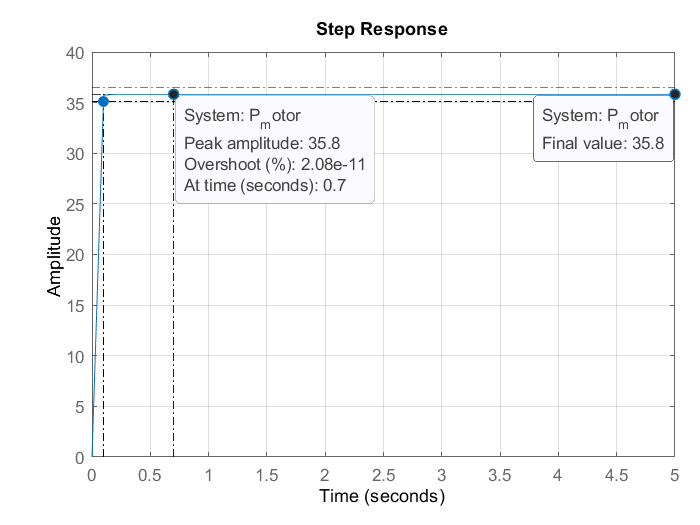
\includegraphics[width=7.5cm]{Matlab/olDCSpeed.png}
		\end{column}%
		\hfill%
		\begin{column}{0.48\textwidth}
			Hasil \textit{Closed-loop}:
			\color{blue}\rule{\linewidth}{4pt}
			\begin{center}
				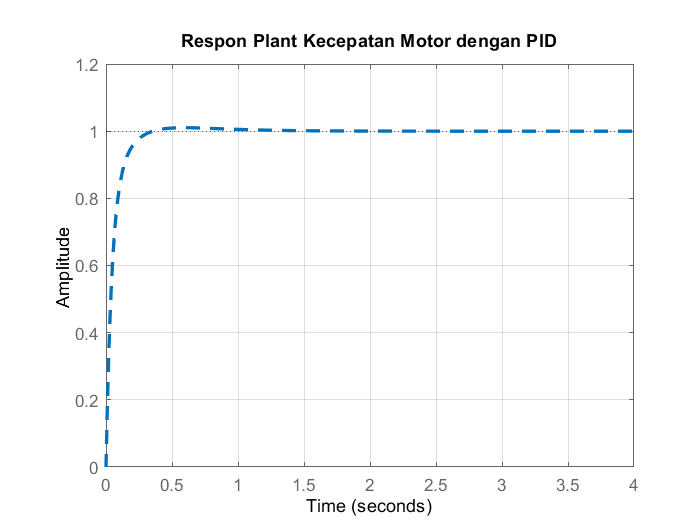
\includegraphics[width=7.5cm]{Matlab/clDCSpeed.png}
			\end{center}
		\end{column}
	\end{columns}
\end{frame}

\begin{frame}{Kendali PID: Kecepatan}
	\begin{columns}[T] % align columns
		\begin{column}{0.48\textwidth}
			Program:
			\color{black}\rule{\linewidth}{4pt}
			\lstinputlisting[language=Matlab]{Matlab/PIDSpeed.m}
		\end{column}%
		\hfill%
		\begin{column}{0.48\textwidth}
			Hasil:
				\color{blue}\rule{\linewidth}{4pt}
			\begin{center}
				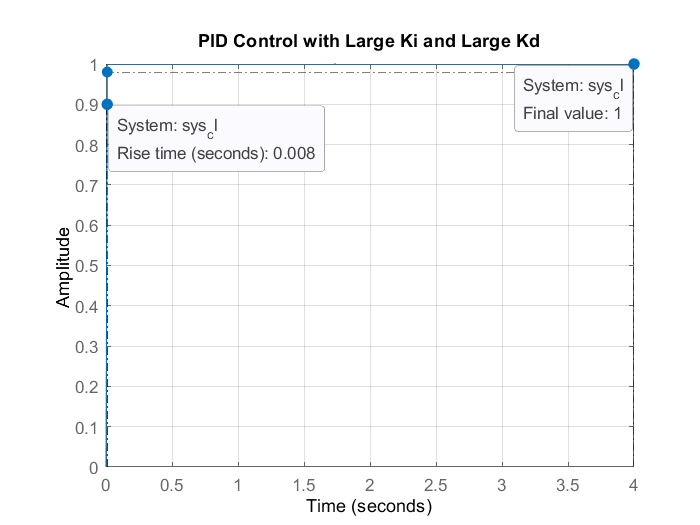
\includegraphics[width=7.5cm]{Matlab/PIDSpeed.png}
			\end{center}
		\end{column}
	\end{columns}
\end{frame}

\begin{frame}{Kendali PID: Posisi}
	\begin{columns}[T] % align columns
		\begin{column}{0.48\textwidth}
			Program:
			\color{black}\rule{\linewidth}{4pt}
			\lstinputlisting[language=Matlab]{Matlab/PIDpos.m}
		\end{column}%
		\hfill%
		\begin{column}{0.48\textwidth}
			Hasil:
			\color{blue}\rule{\linewidth}{4pt}
			\begin{center}
				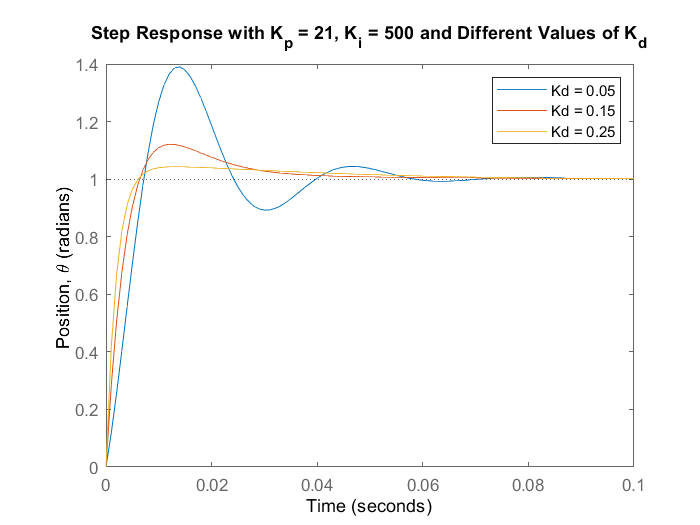
\includegraphics[width=7.5cm]{Matlab/PIDpos.png}
			\end{center}
		\end{column}
	\end{columns}
\end{frame}

\begin{frame}{Simulink}
	\begin{columns}[T] % align columns
		\begin{column}{0.48\textwidth}
			Blok PID:
			\color{black}\rule{\linewidth}{4pt}
			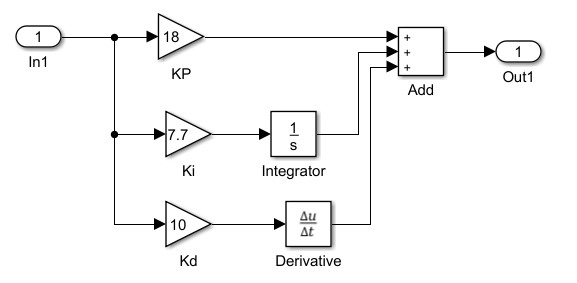
\includegraphics[width=7.5cm]{Matlab/simulink2.jpg}
		\end{column}%
		\hfill%
		\begin{column}{0.48\textwidth}
			Blok Plant Motor DC
			\color{blue}\rule{\linewidth}{4pt}
			\begin{center}
				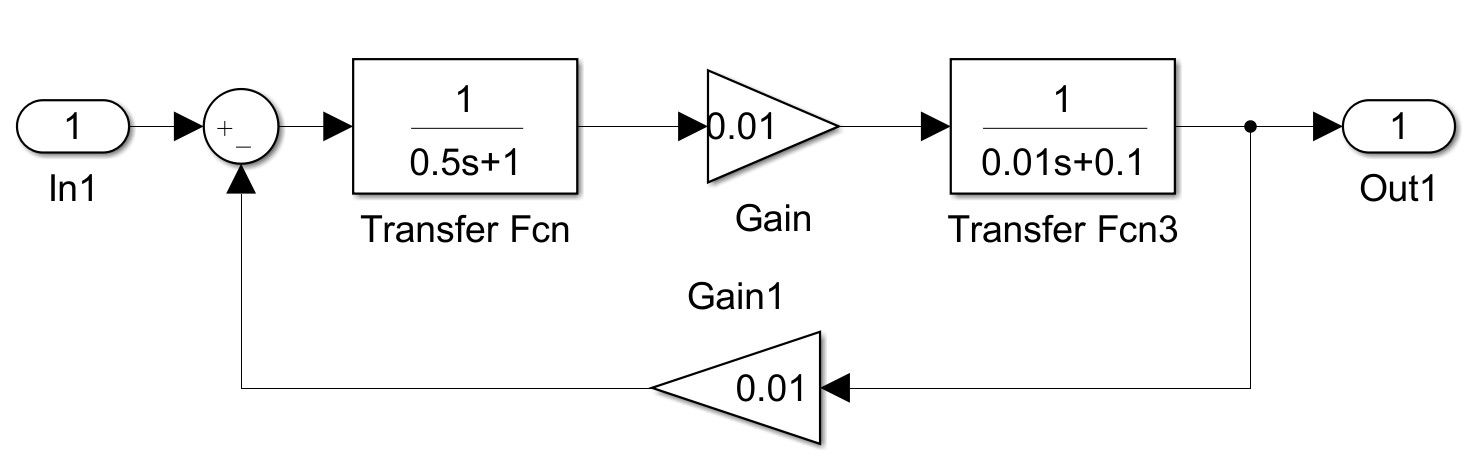
\includegraphics[width=7.5cm]{Matlab/simulink3.jpg}
			\end{center}
		\end{column}
	\end{columns}
\end{frame}

\begin{frame}{Simulink}
	\begin{columns}[T] % align columns
		\begin{column}{0.48\textwidth}
			Blok Simulink
			\color{black}\rule{\linewidth}{4pt}
			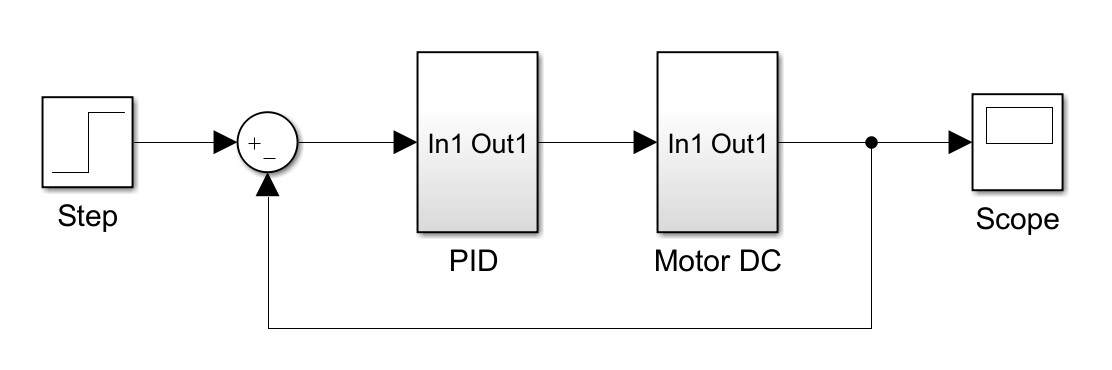
\includegraphics[width=7.5cm]{Matlab/simulink1.jpg}
		\end{column}%
		\hfill%
		\begin{column}{0.48\textwidth}
			Hasil
			\color{blue}\rule{\linewidth}{4pt}
			\begin{center}
				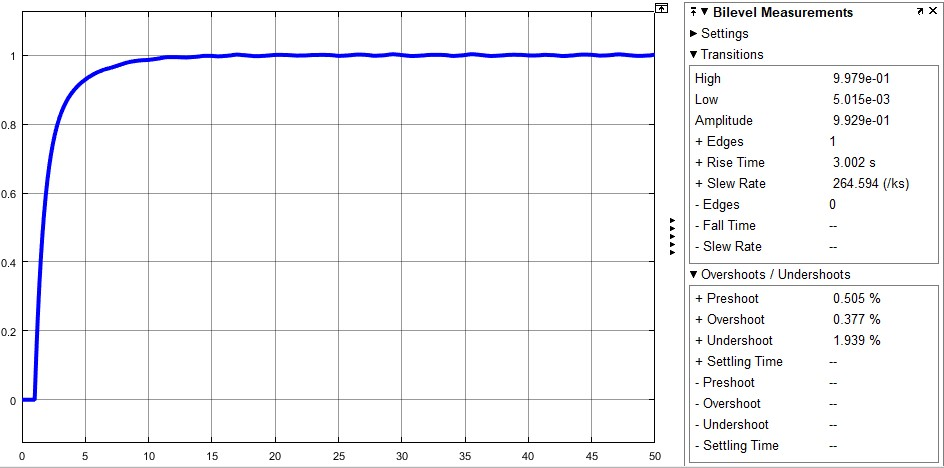
\includegraphics[width=7.5cm]{Matlab/simulink4.jpg}
			\end{center}
		\end{column}
	\end{columns}
\end{frame}

\section{Simulasi LQR}
\begin{frame}[t,fragile]{Simulasi LQR: Kecepatan}
	Klik untuk menjalankan animasi scroll:
	% typeset code into xsavebox `code1'
	\begin{codescroll}[style=C++]{code1}{43}{24}
			%% Mendefinisikan Parameter-parameter yang diperlukan
		J = 0.01;
		b = 0.1;
		K = 0.01;
		R = 1;
		L = 0.5;
		
		%% Matriks State-Space
		
		A = [-b/J    K/J
		-K/L    -R/L];
		B = [0
		1/L];
		C = [1  0];
		D=0;
		
		%% Cek Controllability Sistem
		Co = ctrb(A,B)
		rank(Co)
		
		%% LQR
		Q = [1    0
		0    1];
		R = 1;
		
		K = lqr(A, B, Q, R)
		
		%% Opened Loop Sistem
		sys_ol= ss(A,B,C,D)
		figure(1), step(sys_ol,0:0.01:10)
		grid on
		title('Opened-Loop Kendali Kecepatan'), xlabel('Waktu'),ylabel('Kecepatan')
		
		%% Closed Loop sistem
		A_cl = A-B*K   
		sys_cl= ss(A_cl,B,C,D)
		figure(2), step(sys_cl,0:0.01:10)
		grid on
		title('Closed-Loop Kendali Kecepatan'), xlabel('Waktu'),ylabel('Kecepatan')
	\end{codescroll}
\end{frame}

\begin{frame}[t,fragile]{Simulasi LQR: Posisi}
	Klik untuk menjalankan animasi scroll:
	% typeset code into xsavebox `code1'
	\begin{codescroll}[style=C++]{code1}{43}{24}
		%% Mendefinisikan Parameter-parameter yang diperlukan
		J = 3.2284E-6;
		b = 3.5077E-6;
		K = 0.0274;
		R = 4;
		L = 2.75E-6;
		
		%% Matriks State-Space
		
		A = [0  1       0
		0  -b/J    K/J
		0  -K/L    -R/L];
		B = [0
		0
		1/L];
		C = [1  0   0];
		D=0;
		
		%% Cek Controllability Sistem
		Co = ctrb(A,B)
		rank(Co)
		
		%% LQR
		Q = [1    0    0
		0    1    0
		0    0    1];
		R = 1;
		
		K = lqr(A, B, Q, R)
		
		%% Opened Loop Sistem
		sys_ol= ss(A,B,C,D)
		figure(1), step(sys_ol,0:0.01:10)
		grid on
		title('Opened-Loop Kendali Posisi'), xlabel('Waktu'),ylabel('Sudut')
		
		%% Closed Loop sistem
		A_cl = A-B*K   
		sys_cl= ss(A_cl,B,C,D)
		figure(2), step(sys_cl,0:0.01:10)
		grid on
		title('Closed-Loop Kendali Posisi'), xlabel('Waktu'),ylabel('Sudut')
	\end{codescroll}
\end{frame}

\section{Sistem Mekanikal dan Elektrikal}
\begin{frame}{Komponen-Komponen Utama}
	\begin{columns}[T]
		\begin{column}{0.31\textwidth}
			\begin{center}
				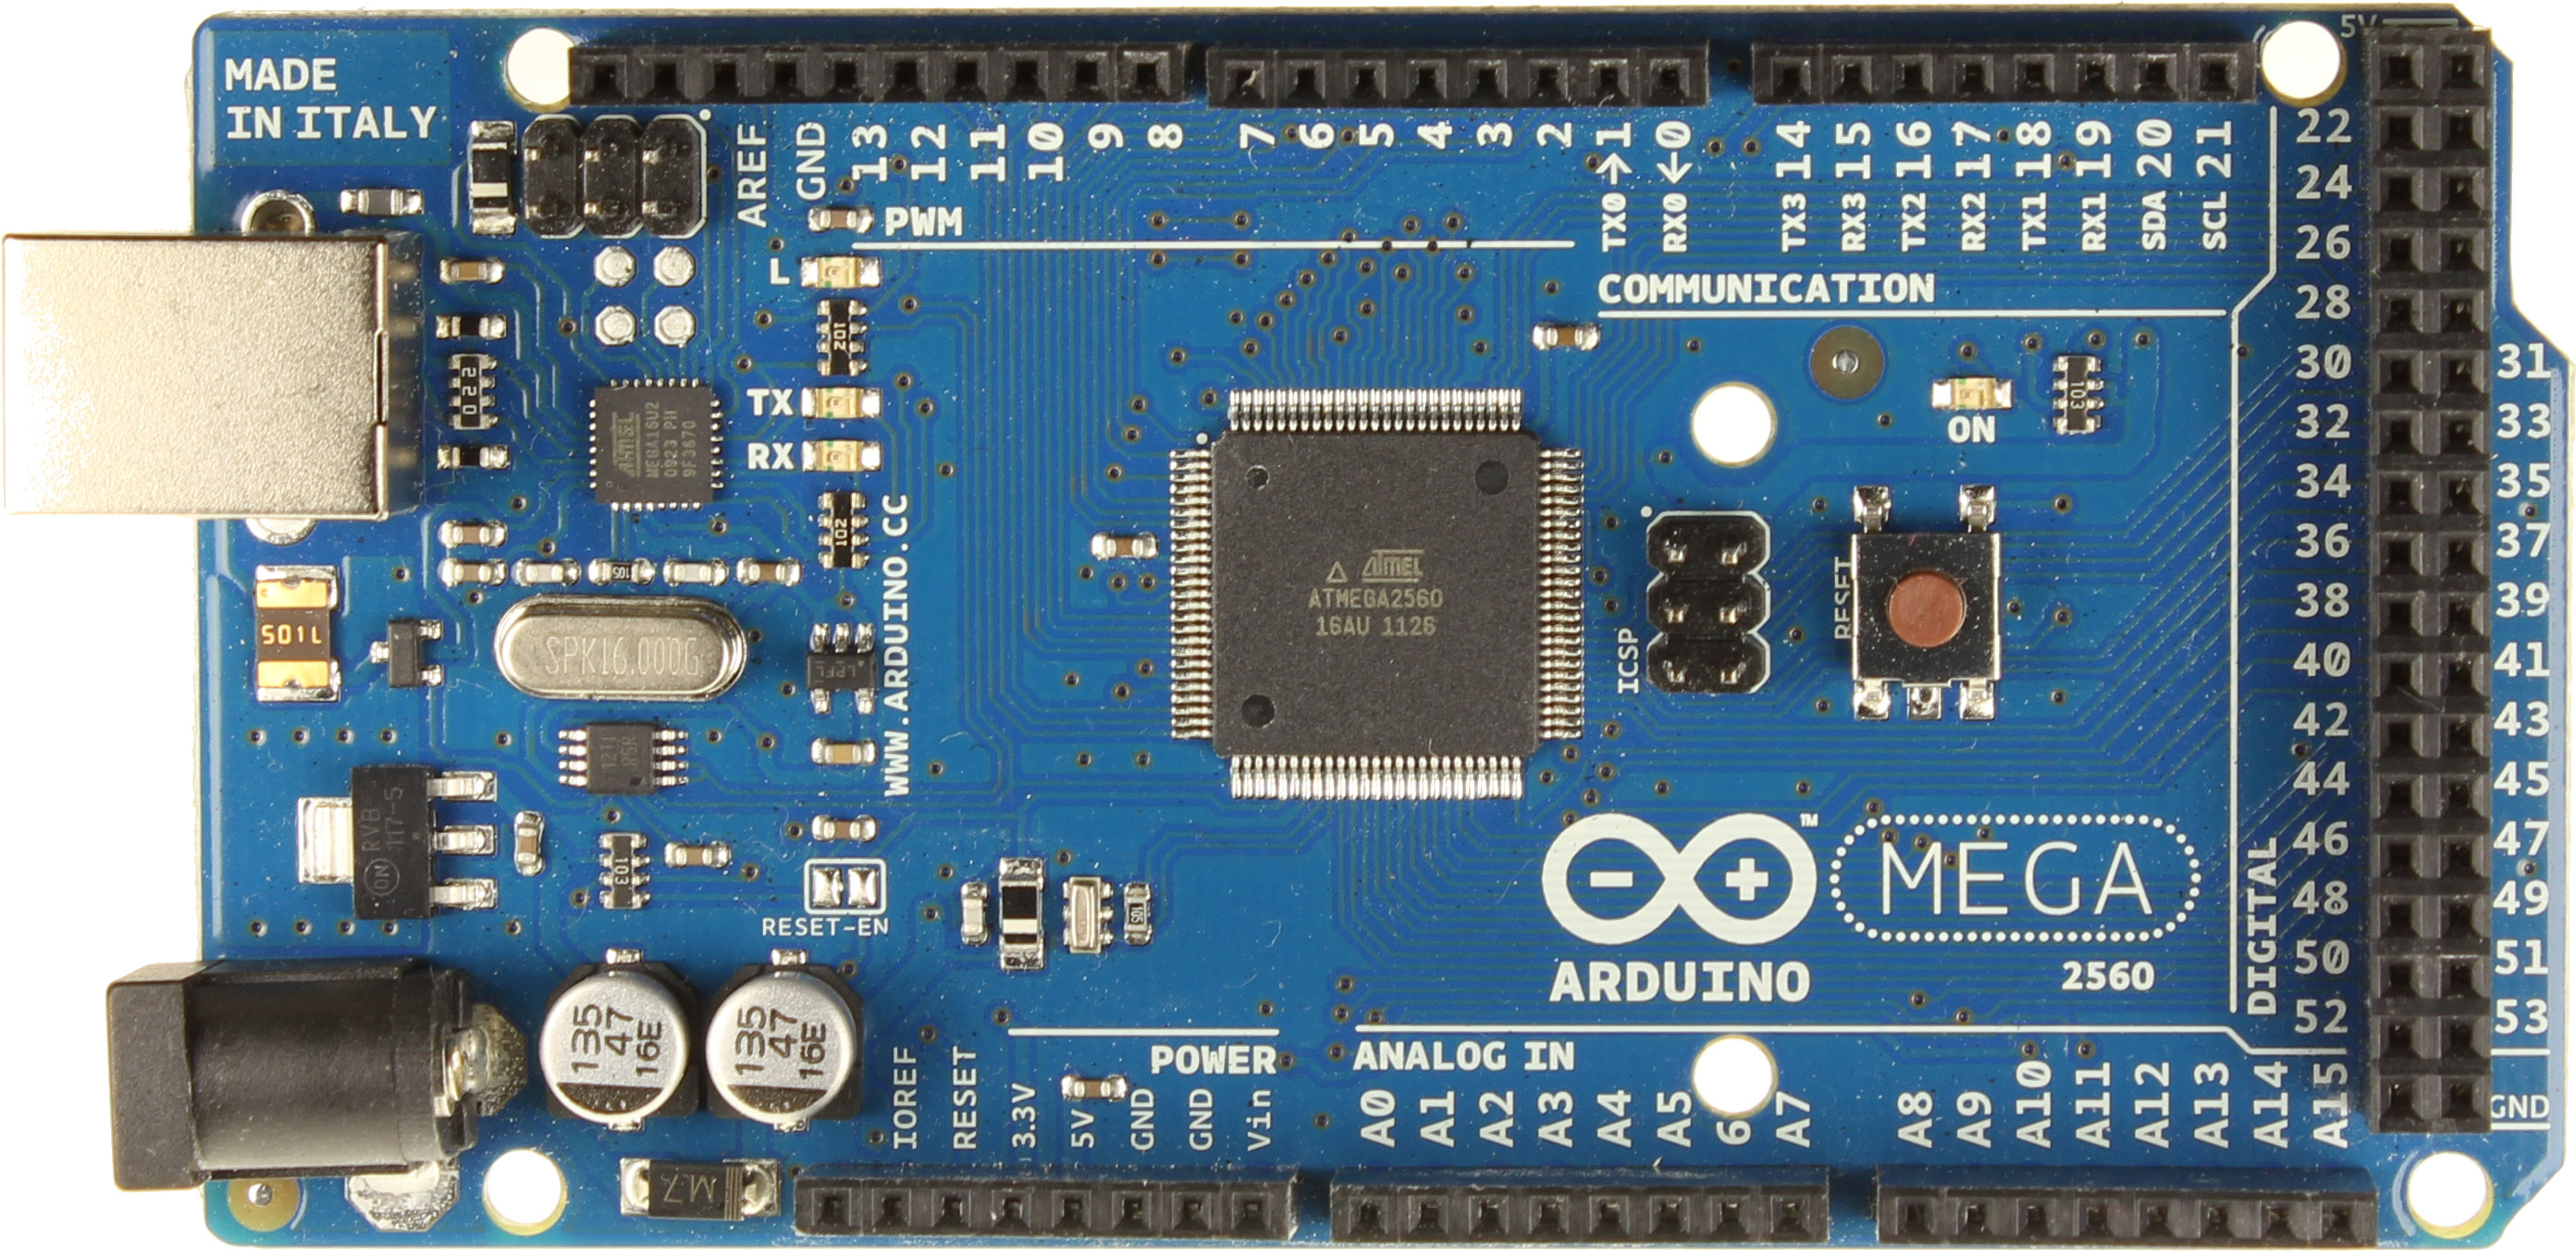
\includegraphics[width=4cm]{Gambar Komponen/MEGA.jpg}
				Arduino Mega\newline\newline
				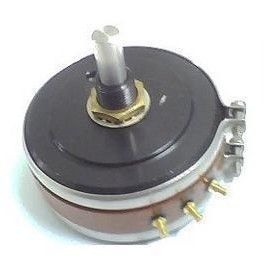
\includegraphics[width=3cm]{Gambar Komponen/POT.jpg}
				Potensiometer $360^o$
			\end{center}
		\end{column}
		\begin{column}{0.31\textwidth}
			\begin{center}
				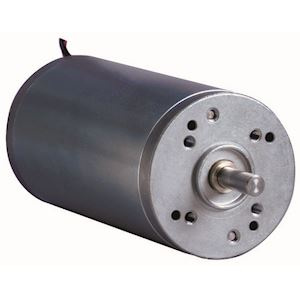
\includegraphics[width=2.5cm]{Gambar Komponen/MOTOR.jpg}
				\newline Motor DC\newline\newline
				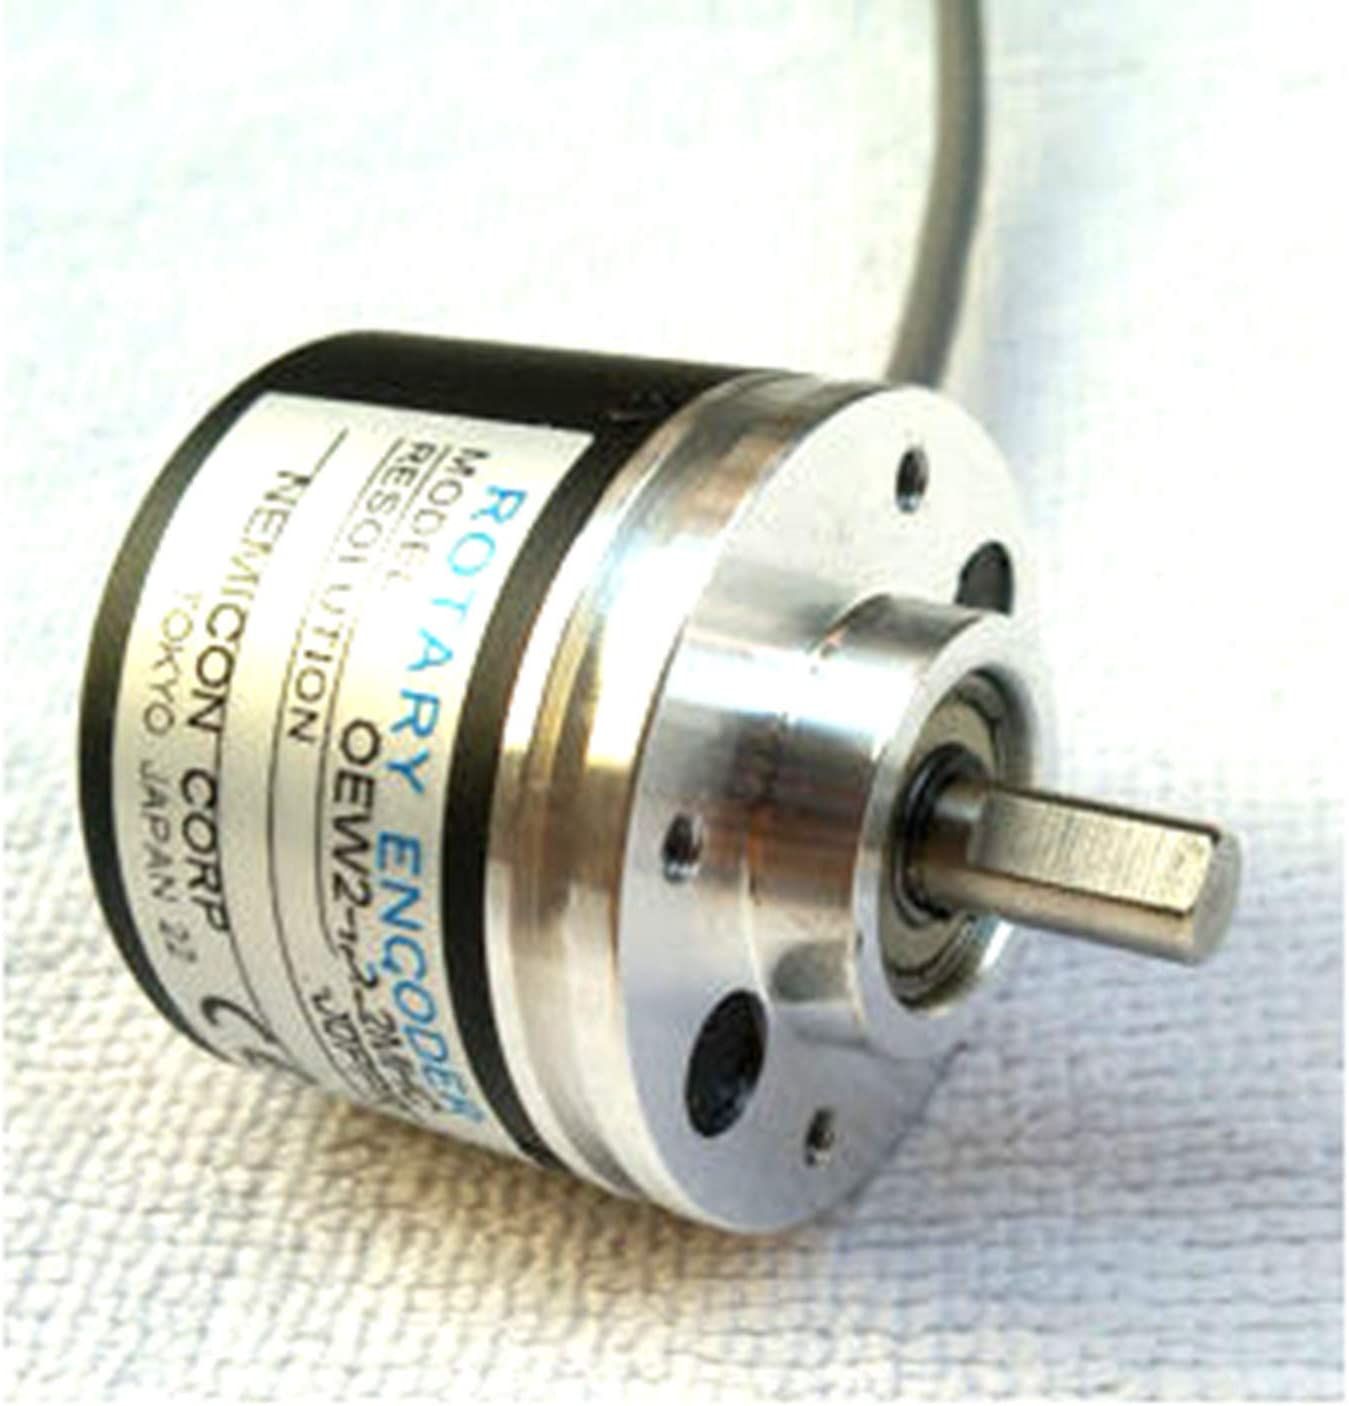
\includegraphics[width=2.5cm]{Gambar Komponen/ENCODER.jpg}
				\newline Rotary Encoder
			\end{center}
		\end{column}
		\begin{column}{0.31\textwidth}
			\begin{center}
				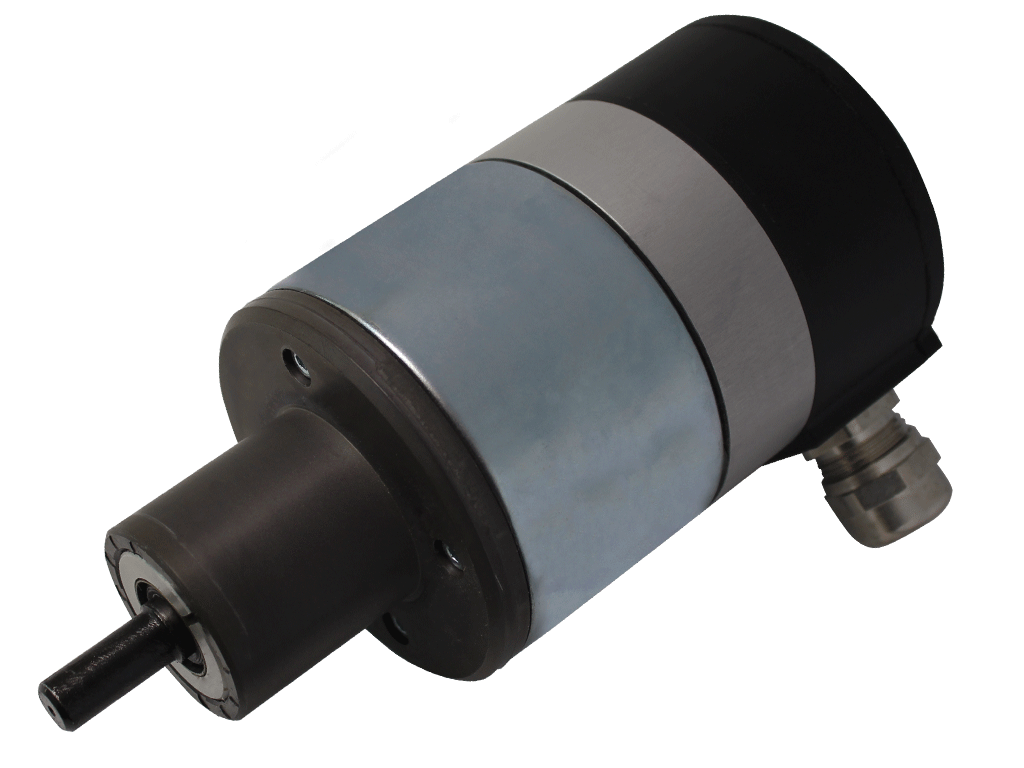
\includegraphics[width=2.5cm]{Gambar Komponen/TACHO.png}
				\newline Tachogenerator
			\end{center}
		\end{column}
	\end{columns}
\end{frame}
\begin{frame}{Diagram Sistem}
	Komponen-komponen utama kemudian disusun menjadi suatu sistem yang ditunjukkan pada diagram sistem seperti yang sudah ditunjukkan di awal.
	\begin{center}
		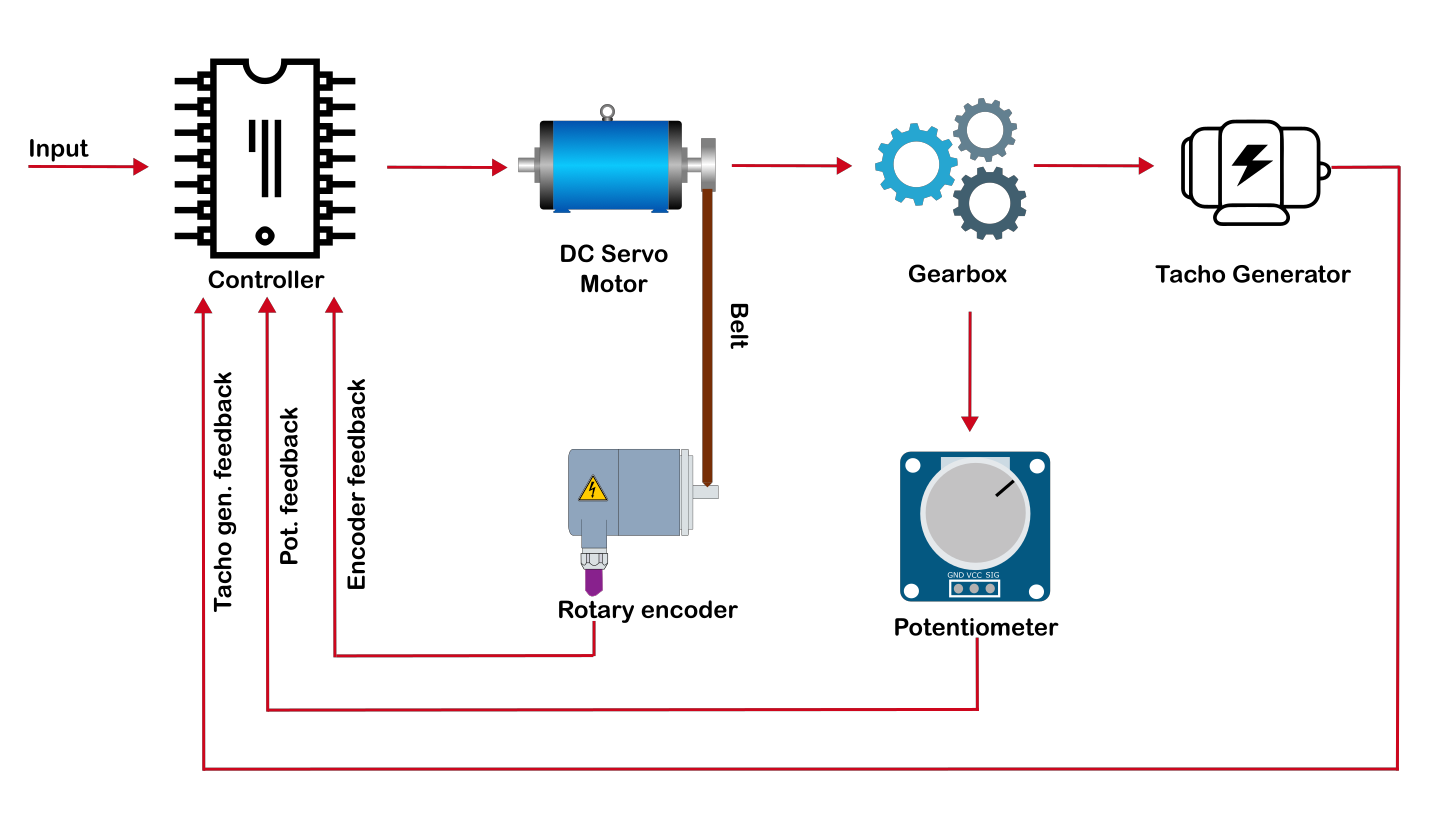
\includegraphics[width=10cm]{Gambar Lain/diagramDCservo.png}
	\end{center}
\end{frame}

\begin{frame}{Konfigurasi Pin-Pin Arduino Mega}
	\begin{columns}[T]
		\begin{column}{0.48\textwidth}
			\centering
			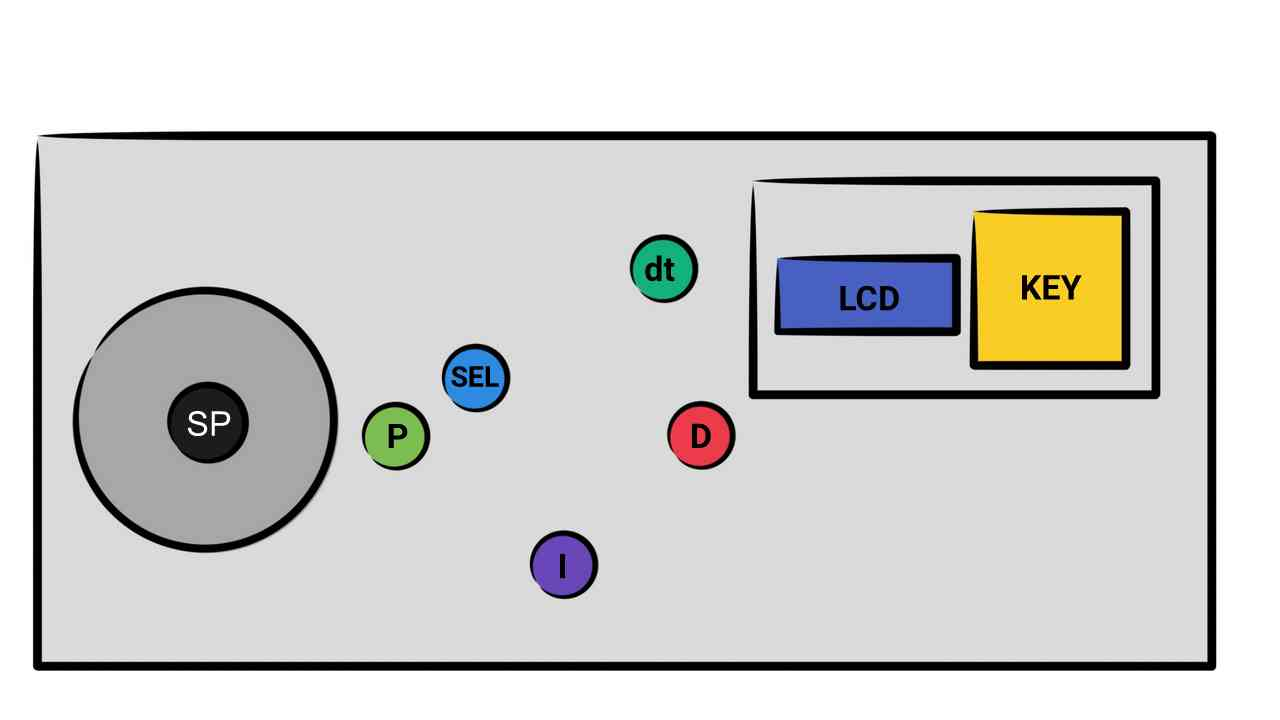
\includegraphics[width=6cm]{Gambar Lain/KONTORU.jpg}
			Kontroler
		\end{column}
		\begin{column}{0.48\textwidth}
			\begin{tabular}{ | m{1cm} | m{2cm}| m{2cm}|} 
				\hline
				\textbf{Input-Output} & \textbf{Fungsi} & \textbf{Pin} \\ 
				\hline
				SP & Set Poin & A7\\ 
				\hline
				P & Proporsional & A5 \\
				\hline
				I & Integral & A8 \\
				\hline
				D & Derivatif & A6 \\
				\hline
				SEL & \textit{Selector} & 34, 32, 30 \\
				\hline
				dt & \textit{Time Sampling} & A4 \\
				\hline
				LCD & LCD & 0, 1 \\
				\hline
				KEY & Keypad & 52, 50, 48, 46, 44, 42, 40, 38 \\
				\hline
			\end{tabular}
		\end{column}
	\end{columns}
\end{frame}

\begin{frame}{Desain 3D}
	\begin{columns}[T] % align columns
		\begin{column}{0.48\textwidth}
			Board PCB
			\color{black}\rule{\linewidth}{4pt}
			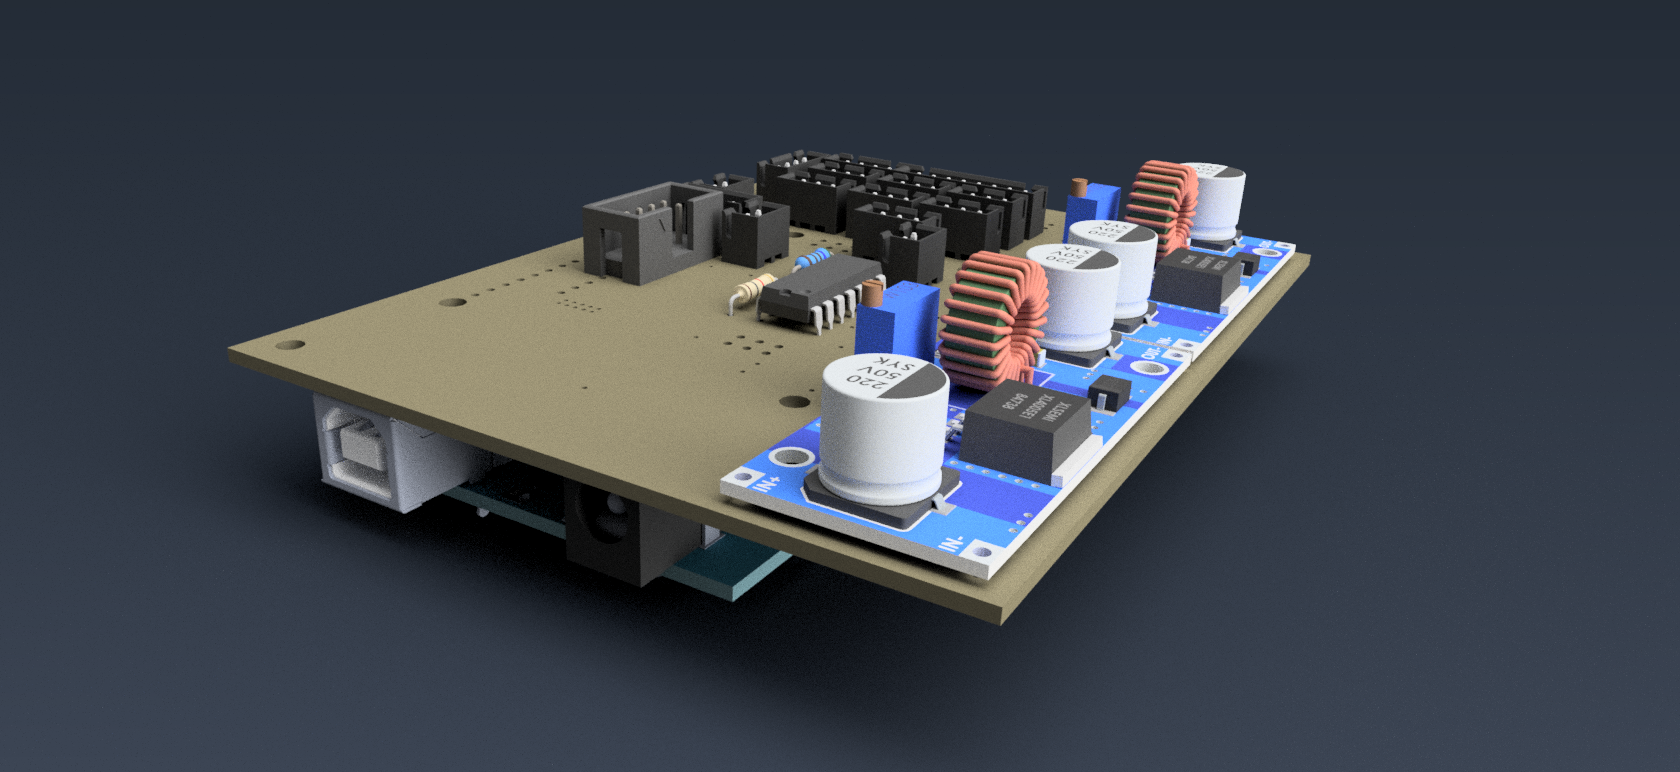
\includegraphics[width=7.5cm]{Render/Main Board_v3 (Home).png}
		\end{column}%
		\hfill%
		\begin{column}{0.48\textwidth}
			Alat
			\color{blue}\rule{\linewidth}{4pt}
			\begin{center}
				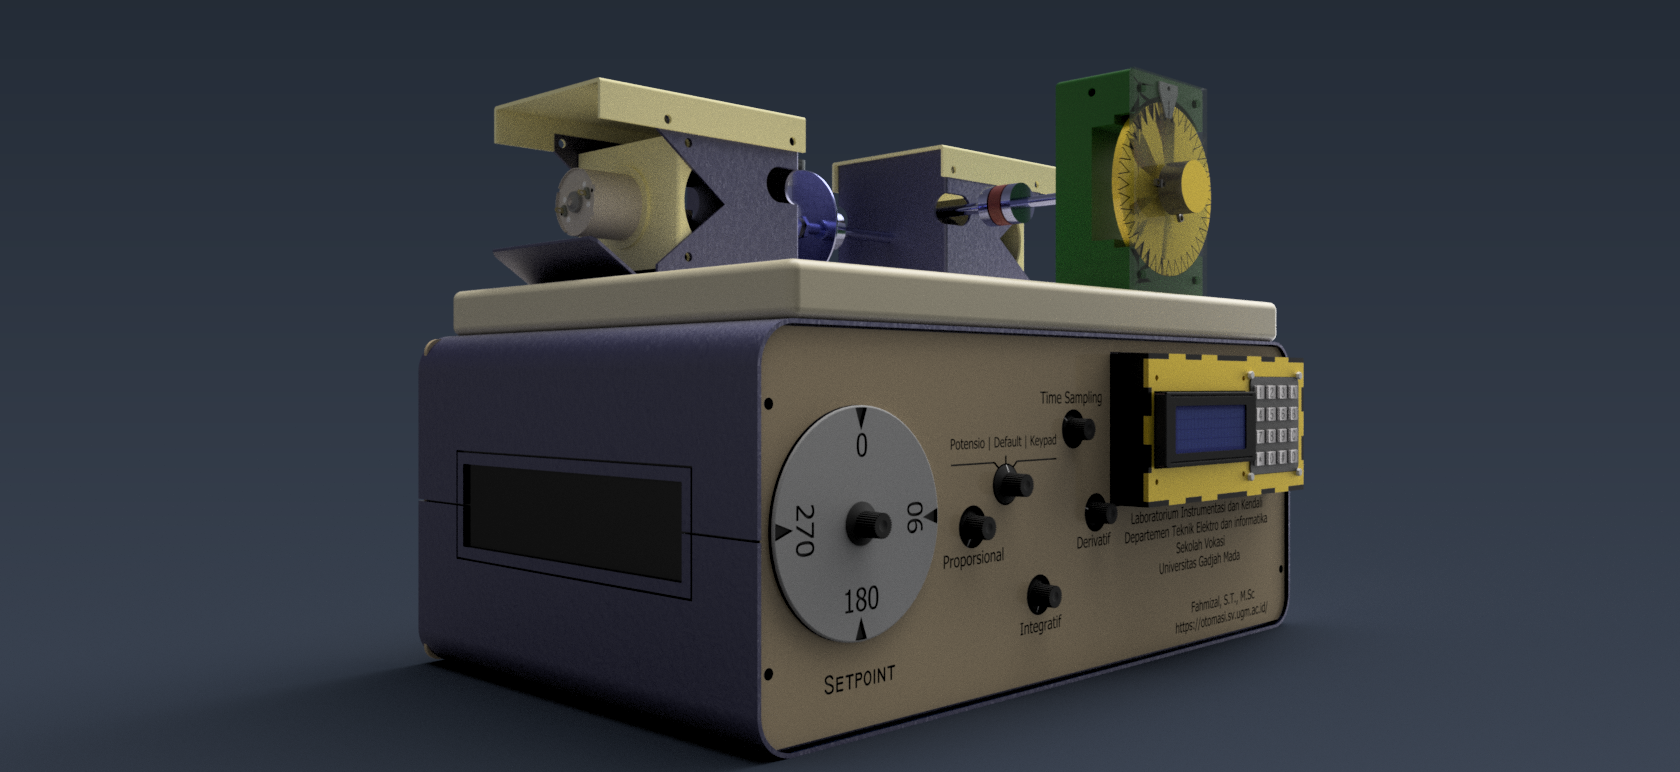
\includegraphics[width=7.5cm]{Render/Feedback Actuator UNIT ES151(Home).png}
			\end{center}
		\end{column}
	\end{columns}
\end{frame}

\begin{frame}{Tampilan Alat}
	\begin{columns}[T] % align columns
		\begin{column}{0.48\textwidth}
			Tampak Depan
			\color{black}\rule{\linewidth}{4pt}
			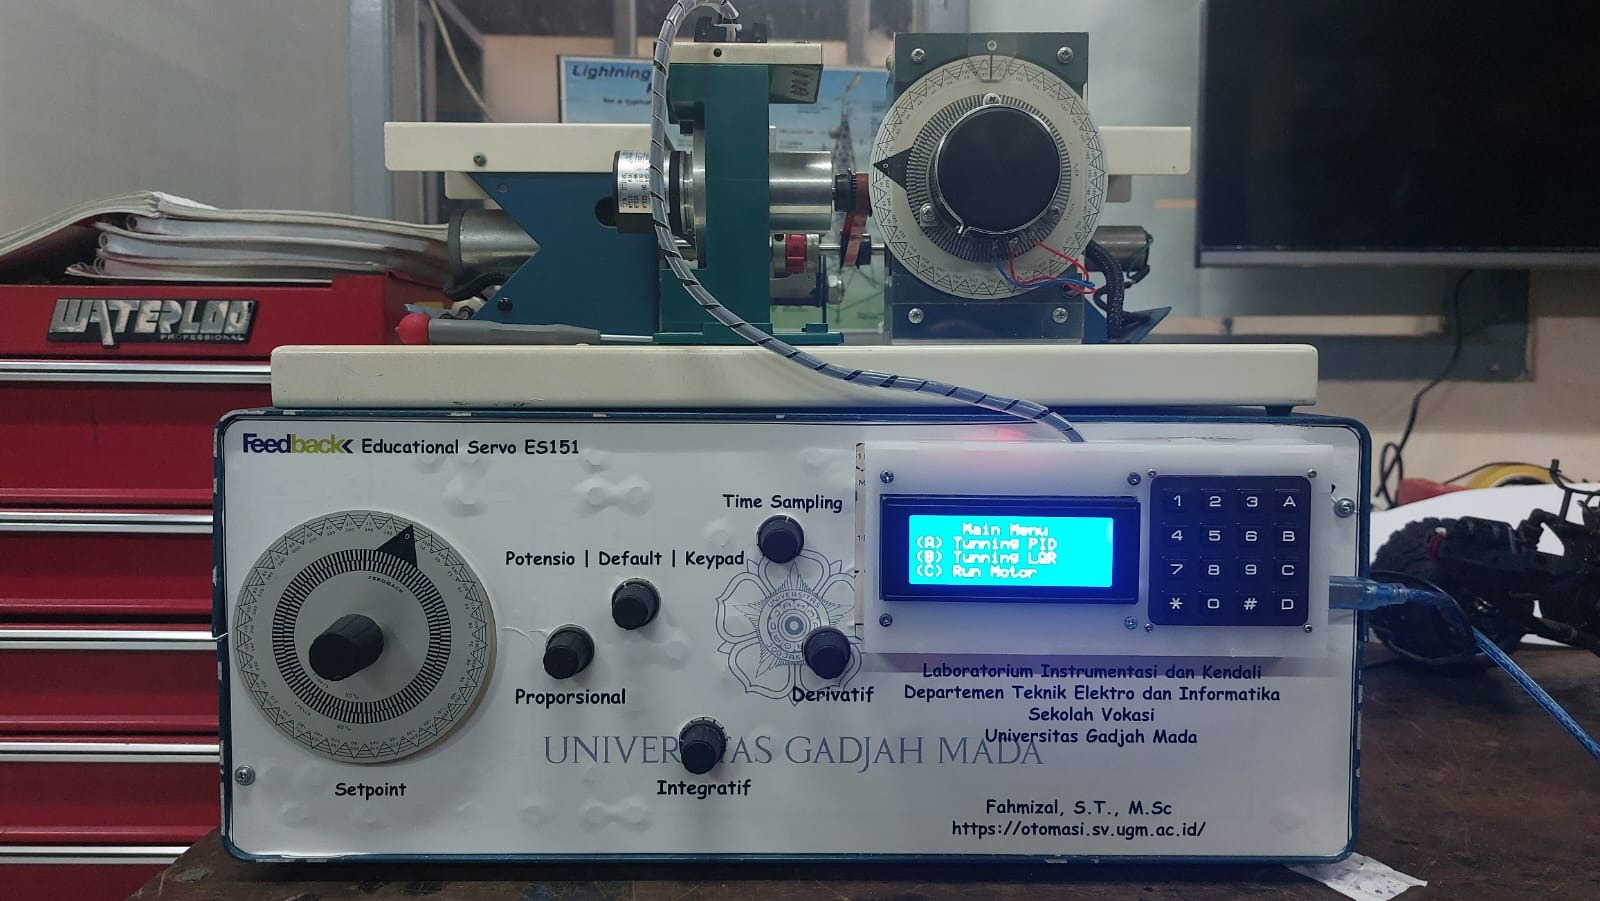
\includegraphics[width=7.5cm]{Gambar Lain/TampakDepan.jpeg}
		\end{column}%
		\hfill%
		\begin{column}{0.48\textwidth}
			Tampak Atas
			\color{blue}\rule{\linewidth}{4pt}
			\begin{center}
				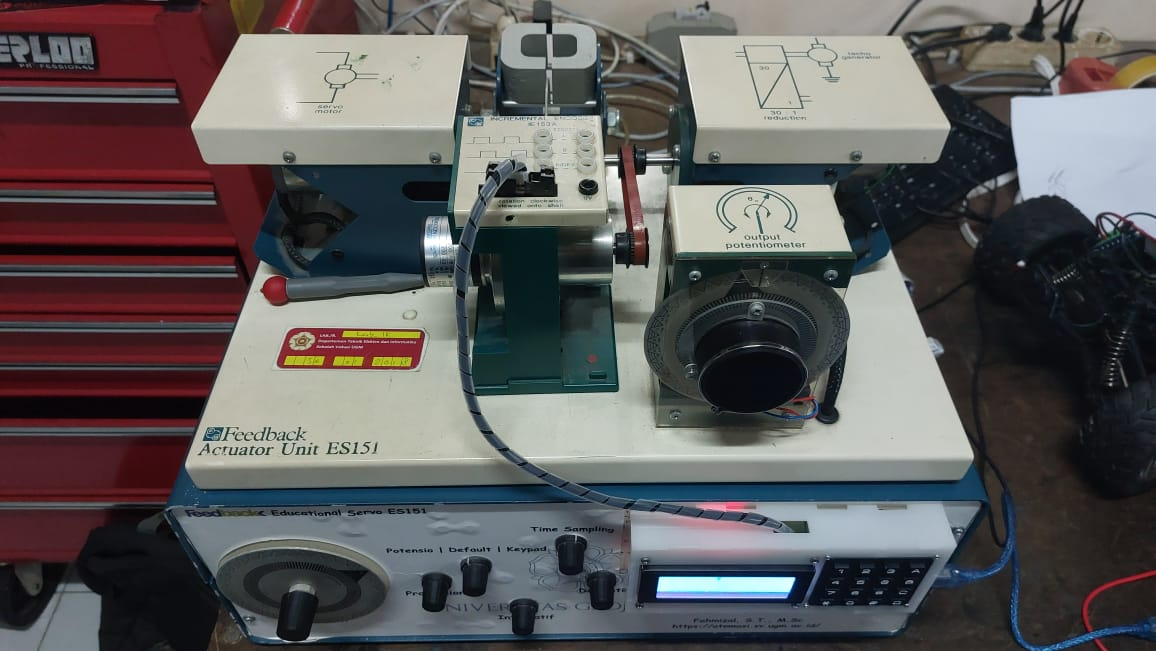
\includegraphics[width=7.5cm]{Gambar Lain/TampakAtas.jpeg}
			\end{center}
		\end{column}
	\end{columns}
\end{frame}

\section{Desain GUI}

\begin{frame}{Percobaan Identifikasi Sistem}
	\begin{columns}[T] % align columns
		\begin{column}{0.48\textwidth}
			Grafik Input dan Output
			\color{black}\rule{\linewidth}{4pt}
			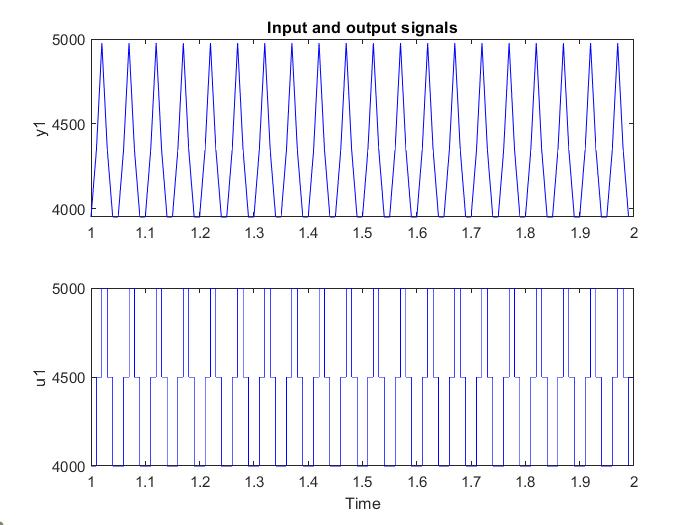
\includegraphics[width=7.5cm]{Coba Sistem Identification/timeplot.jpg}
		\end{column}%
		\hfill%
		\begin{column}{0.48\textwidth}
			Transfer Function
			\color{blue}\rule{\linewidth}{4pt}
			\begin{center}
				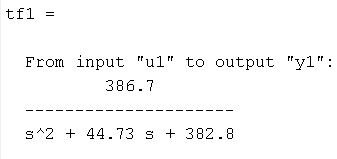
\includegraphics[width=7.5cm]{Coba Sistem Identification/hasiltf1.png}
			\end{center}
		\end{column}
	\end{columns}
\end{frame}

\begin{frame}{Percobaan Identifikasi Sistem}
	\begin{columns}[T] % align columns
		\begin{column}{0.48\textwidth}
			Step Response
			\color{black}\rule{\linewidth}{4pt}
			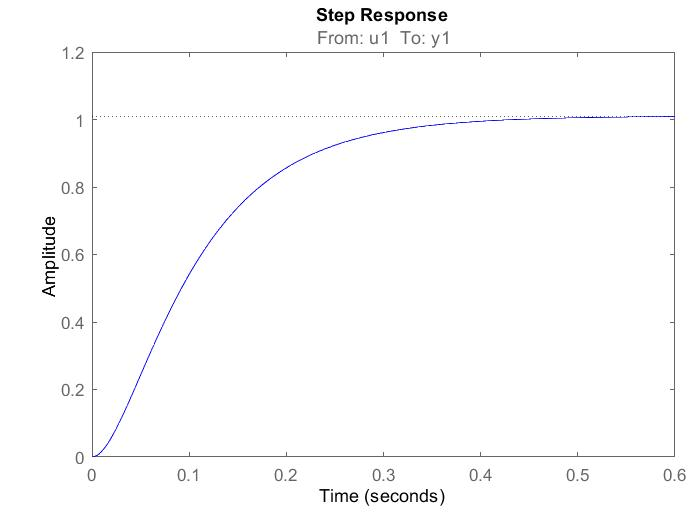
\includegraphics[width=7.5cm]{Coba Sistem Identification/tf1.jpg}
		\end{column}%
		\hfill%
		\begin{column}{0.48\textwidth}
			State Space
			\color{blue}\rule{\linewidth}{4pt}
			\begin{center}
				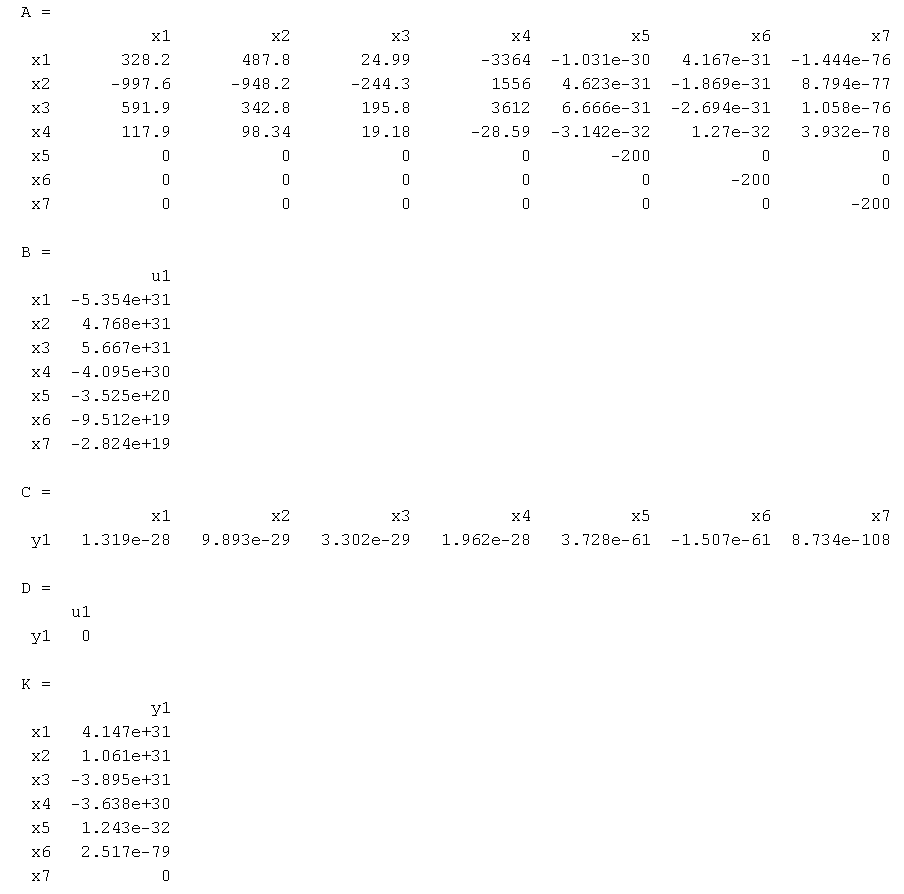
\includegraphics[width=6cm]{Coba Sistem Identification/ss1.png}
			\end{center}
		\end{column}
	\end{columns}
\end{frame}

\begin{frame}{GUI Python TKinter}
	\centering
	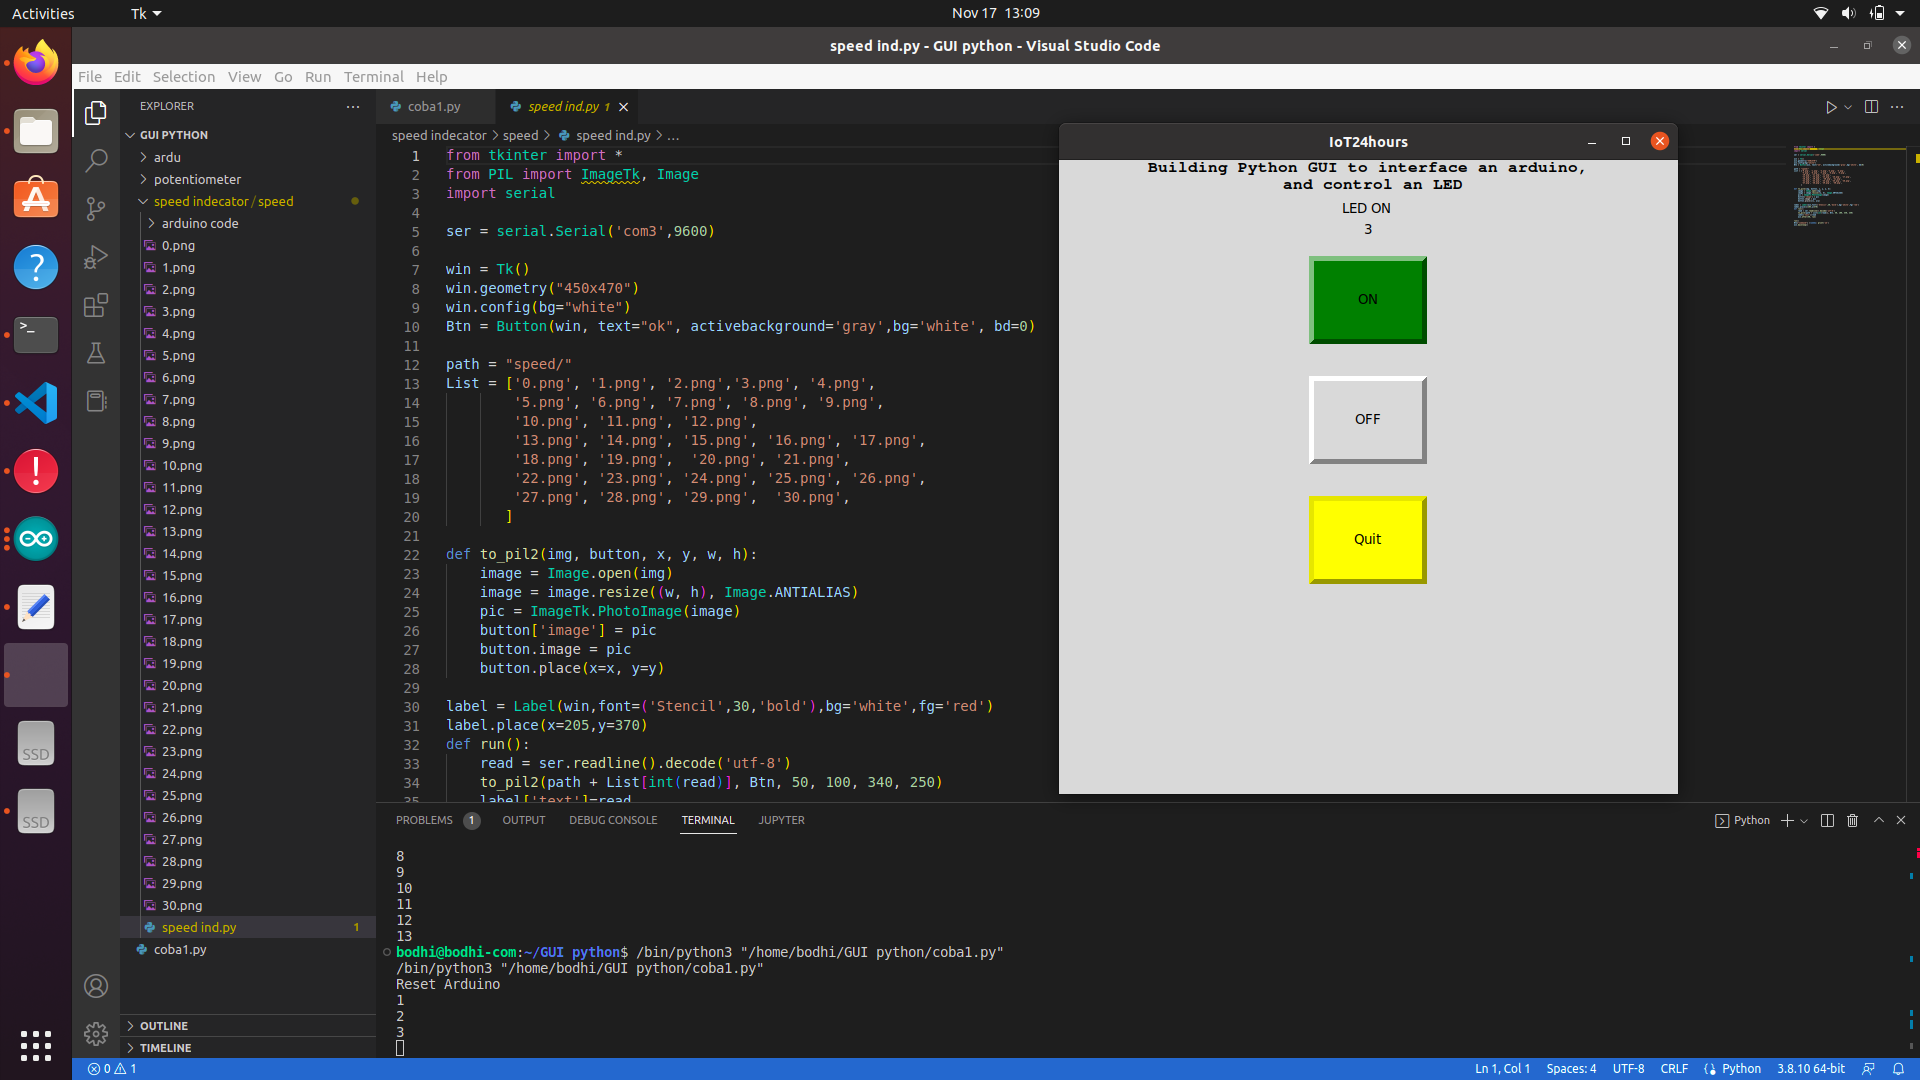
\includegraphics[width=10cm]{Gambar Lain/guitkinter.png}
\end{frame}

%%%%%%%%%%%%%%%%%%%%%%%%%%%%%%
%\section{Simulasi-Simulasi Lainnya}

%\begin{frame}{Simulasi DC Motor Encoder Menggunakan Proteus}
%	\centering
%	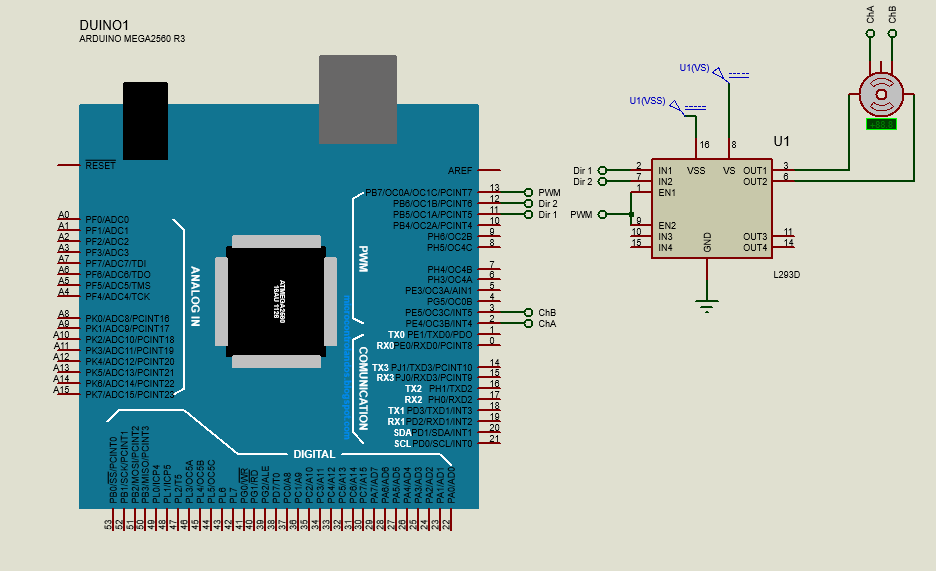
\includegraphics[width=10.0cm]{Gambar Lain/proteus encoder.png}
%\end{frame}

%\begin{frame}{Simulasi PID Analog Di Proteus}
%	\centering
%	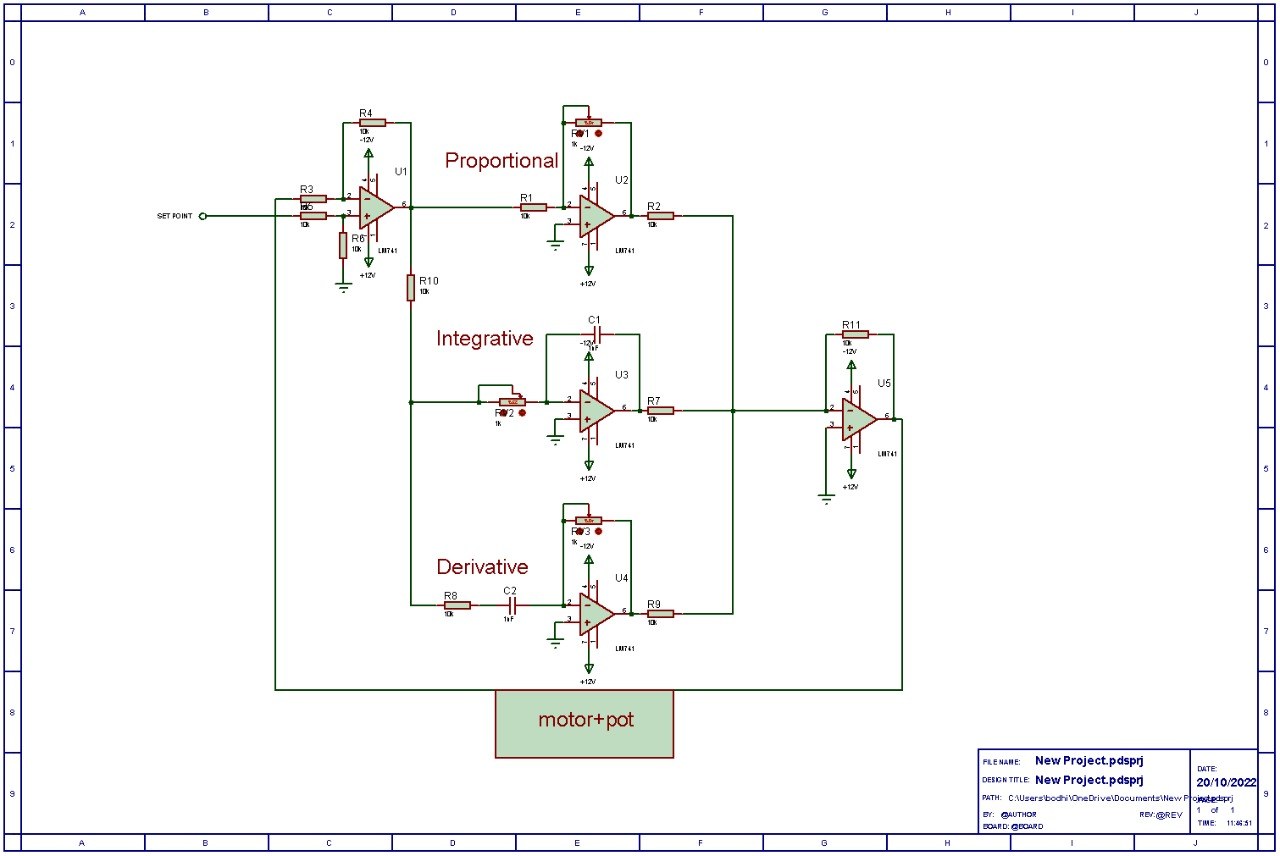
\includegraphics[width=10.0cm]{Gambar Lain/analogpid.jpeg}
%\end{frame}

%\begin{frame}{Simulasi Motor DC Dengan H-Bridge Mosfet Menggunakan Proteus}
%	\centering
%	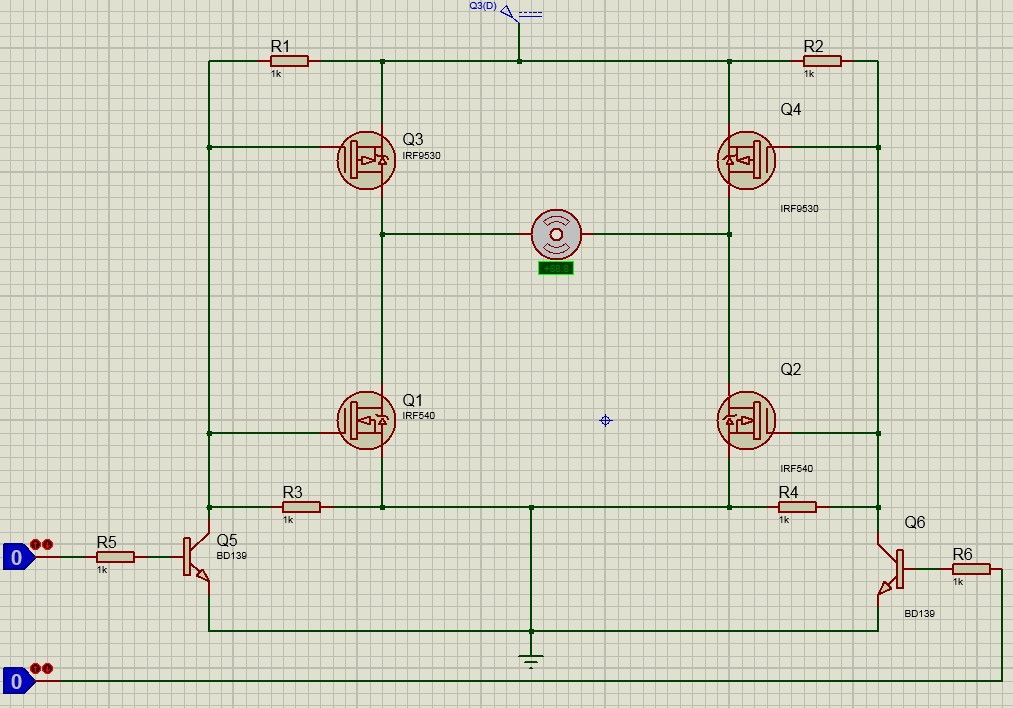
\includegraphics[width=10.0cm]{Gambar Lain/h-bridge mosfet.jpg}
%\end{frame}

%\begin{frame}{Video Simulasi Motor DC dengan H-Bridge Mosfet}
%	\centering
%	\includemovie{4.5in}{2.5in}{Video/h-bridge mosfet compressed.mp4}
%\end{frame}

%\begin{frame}{Diagram Labview}
%	\centering
%	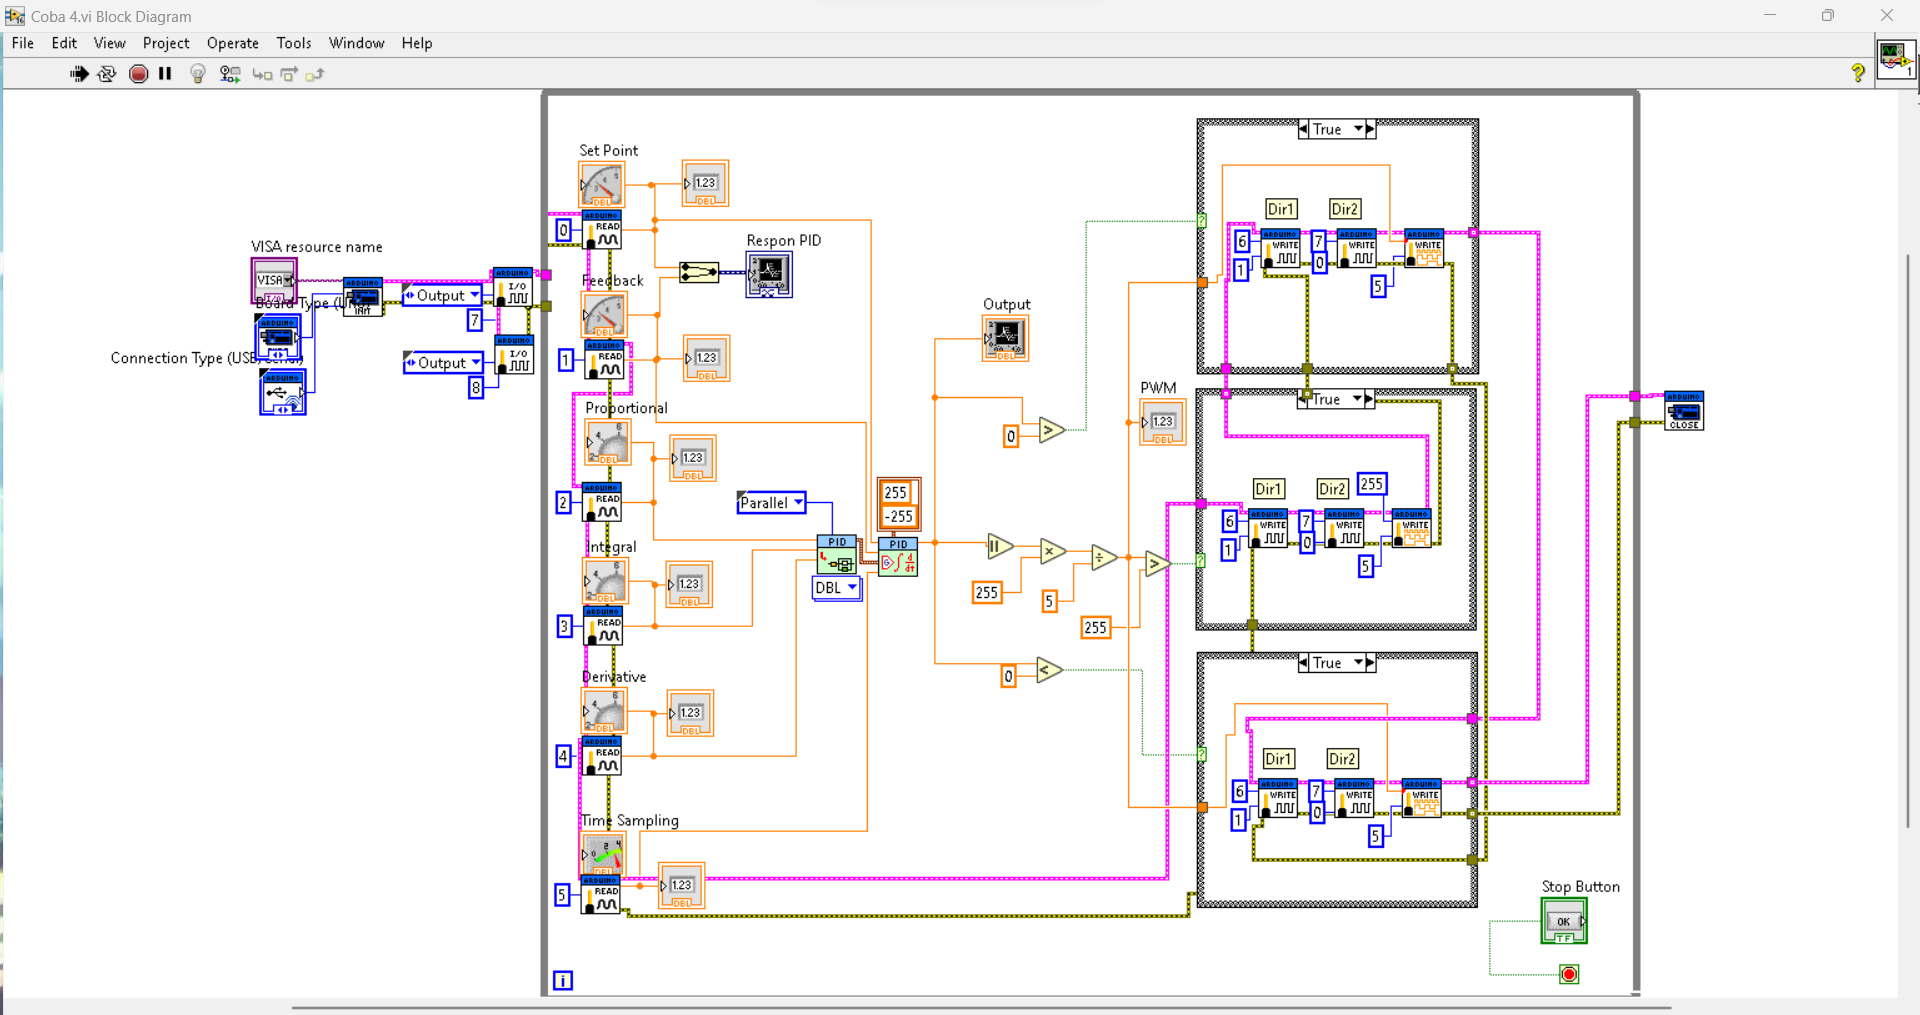
\includegraphics[width=10cm]{Gambar Lain/labview1.png}
%\end{frame}
%
%\begin{frame}{Tampilan GUI Labview}
%	\centering
%	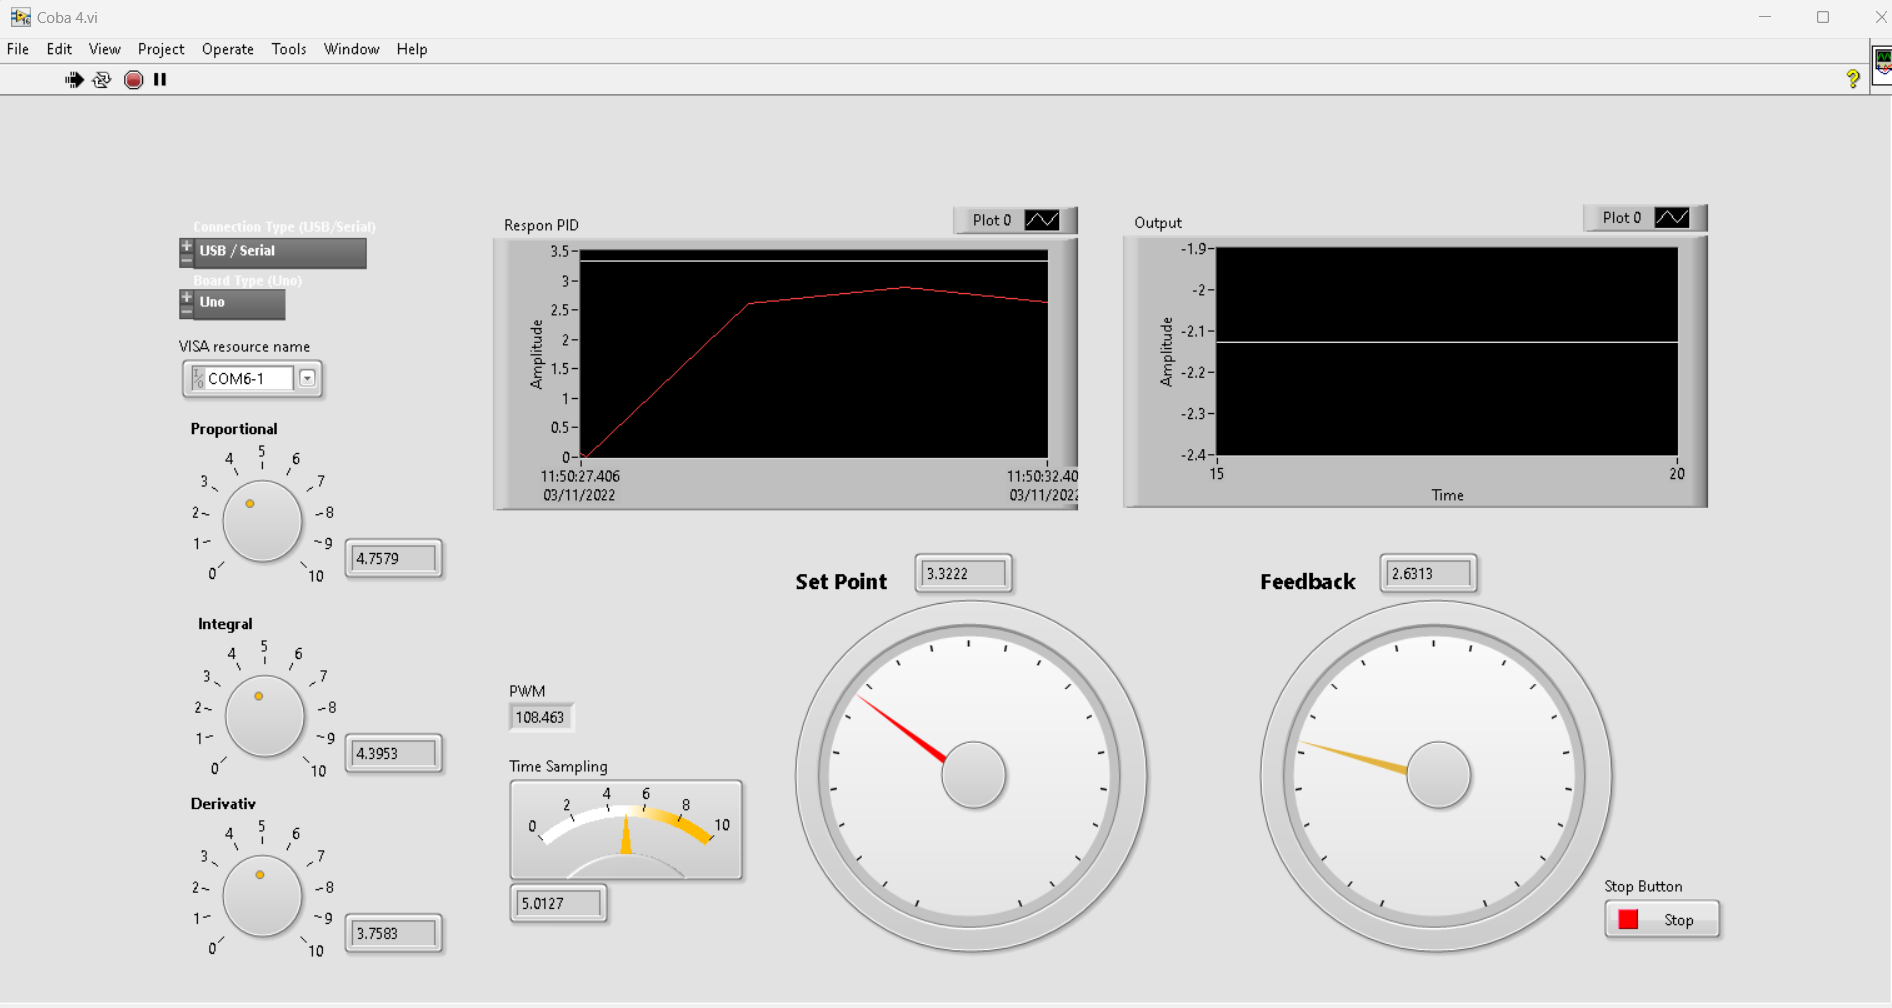
\includegraphics[width=10cm]{Gambar Lain/labview2.png}
%\end{frame}
%
%\begin{frame}{Video LabView}
%	\centering
%	\movie{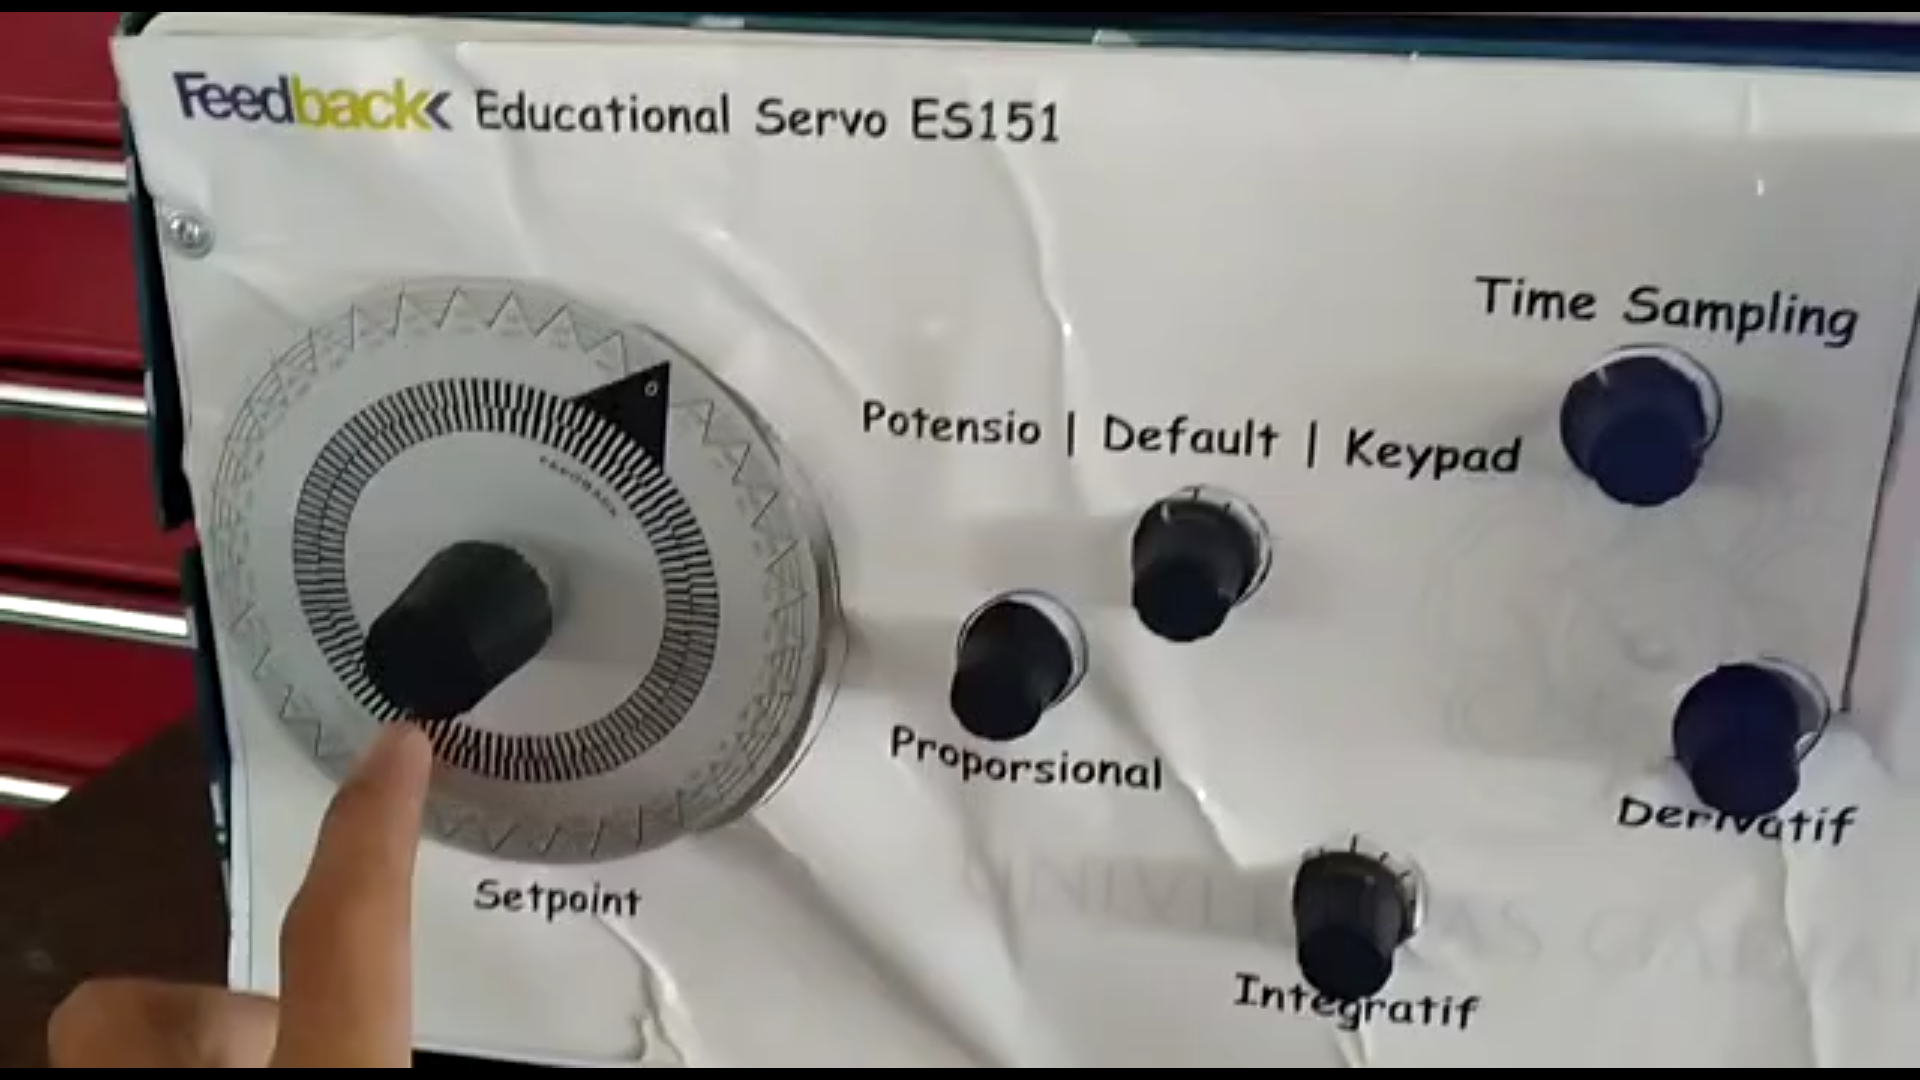
\includegraphics[width=4.5in]{Thumbnail/labview.png}}{Video/LABVIEW.mp4}
%\end{frame}
%
%\begin{frame}{GUI Matlab-Arduino}
%	\centering
%	\includegraphics[width=10cm]{Hasil Matlab/GUI MAtlab 1.png}
%\end{frame}
%
%\begin{frame}{Tampilan GUI Matlab-Arduino}
%	\centering
%	\includegraphics[width=10cm]{Hasil Matlab/GUI MAtlab arduino.png}
%\end{frame}
%
%\begin{frame}{Kode Program Pada Matlab}
%	\lstinputlisting[language=Matlab]{Hasil Matlab/Program1.m}
%\end{frame}
%
%\begin{frame}{Kode Program Pada Matlab}
%	\lstinputlisting[language=Matlab]{Hasil Matlab/Program2.m}
%\end{frame}
%
%\begin{frame}{Video Simulasi GUI Matlab-Arduino}
%	\centering
%	\movie{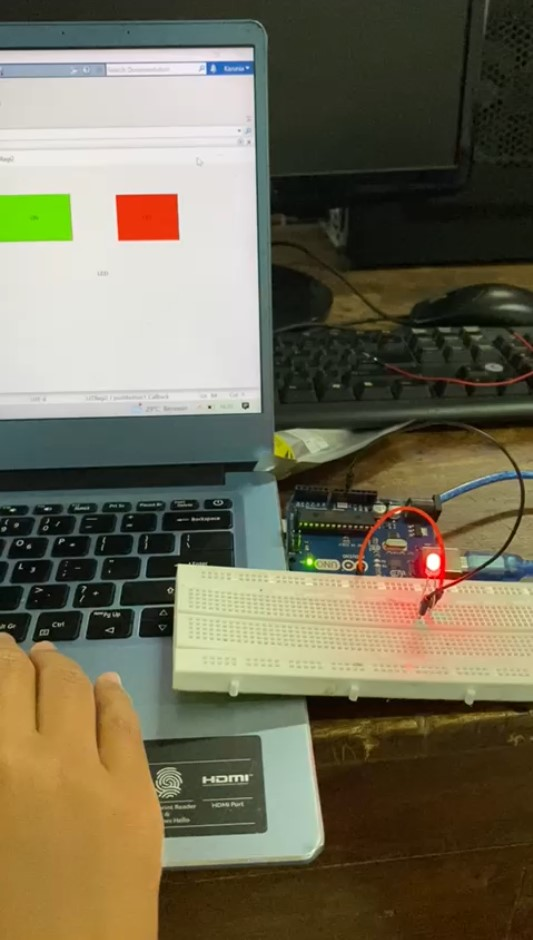
\includegraphics[height=2.8in]{Thumbnail/matlab gui.jpg}}{Video/MatlabGUI.mp4}
%\end{frame}

% \begin{frame}{\textit{Interface PID Controller on Arduino Board With Simulink}}
% 	\begin{columns}[T] % align columns
% 		\begin{column}{0.48\textwidth}
% 			Blok Simulink
% 			\color{black}\rule{\linewidth}{4pt}
% 			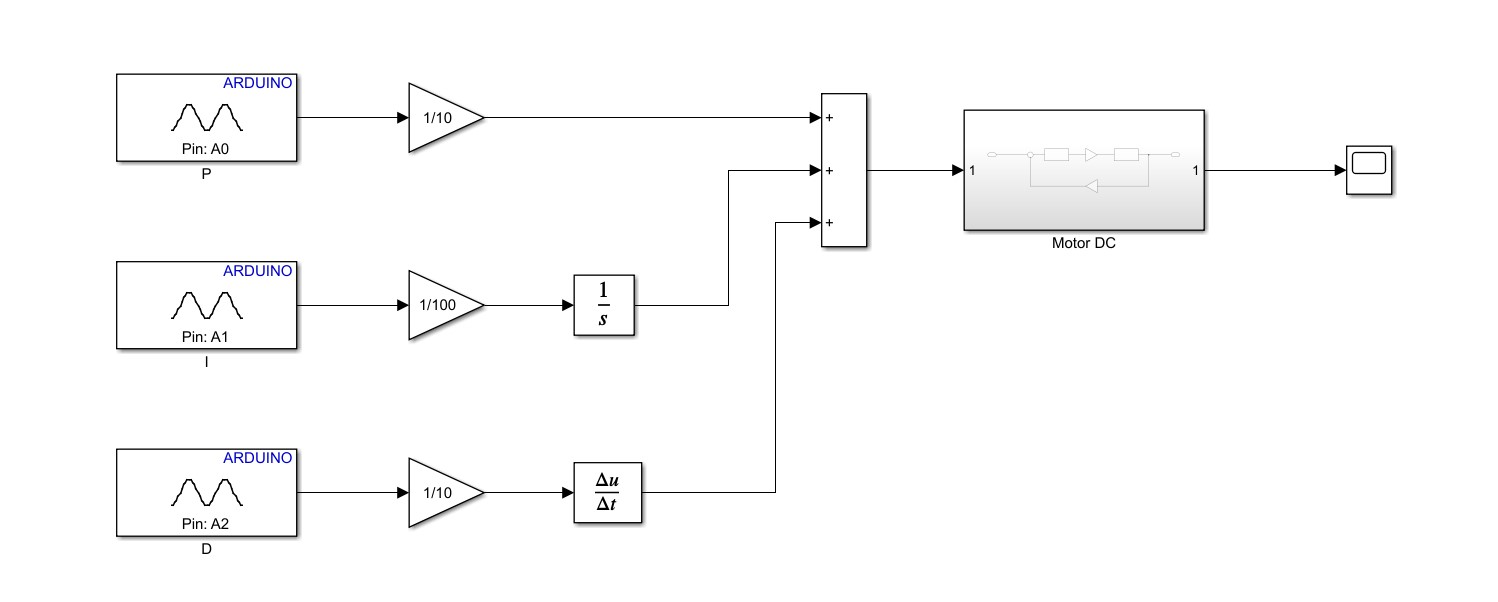
\includegraphics[width=7.5cm]{Gambar Lain/asimulink_pid.jpg}
% 		\end{column}%
% 		\hfill%
% 		\begin{column}{0.48\textwidth}
% 			Hasil
% 			\color{blue}\rule{\linewidth}{4pt}
% 			\begin{center}
% 				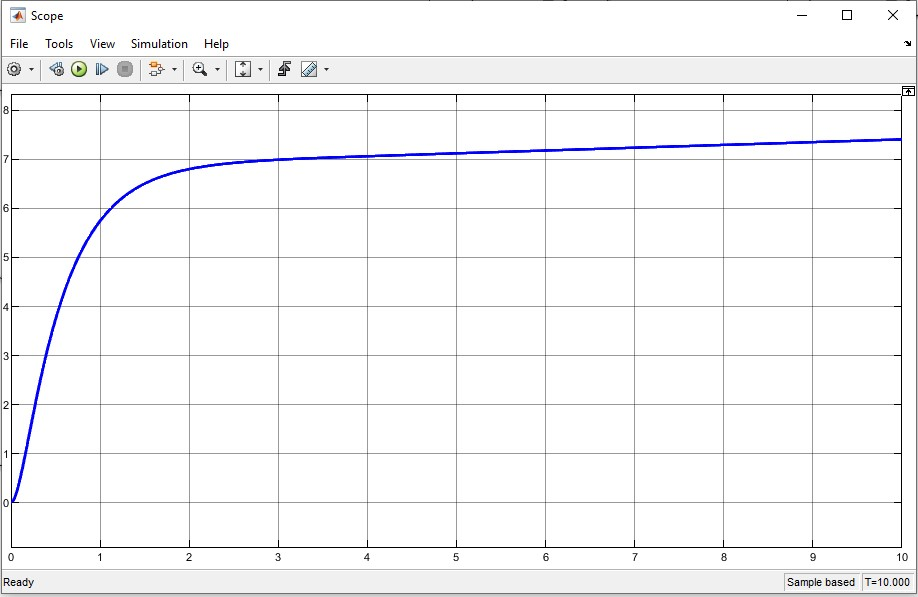
\includegraphics[width=7.5cm]{Hasil Matlab/scopesys.jpg}
% 			\end{center}
% 		\end{column}
% 	\end{columns}
% \end{frame}

%\begin{frame}{\textit{Interface PID Controller on Arduino Board With Simscape}}
%	\begin{columns}[T] % align columns
%		\begin{column}{0.48\textwidth}
%			Blok Simscape
%			\color{black}\rule{\linewidth}{4pt}
%			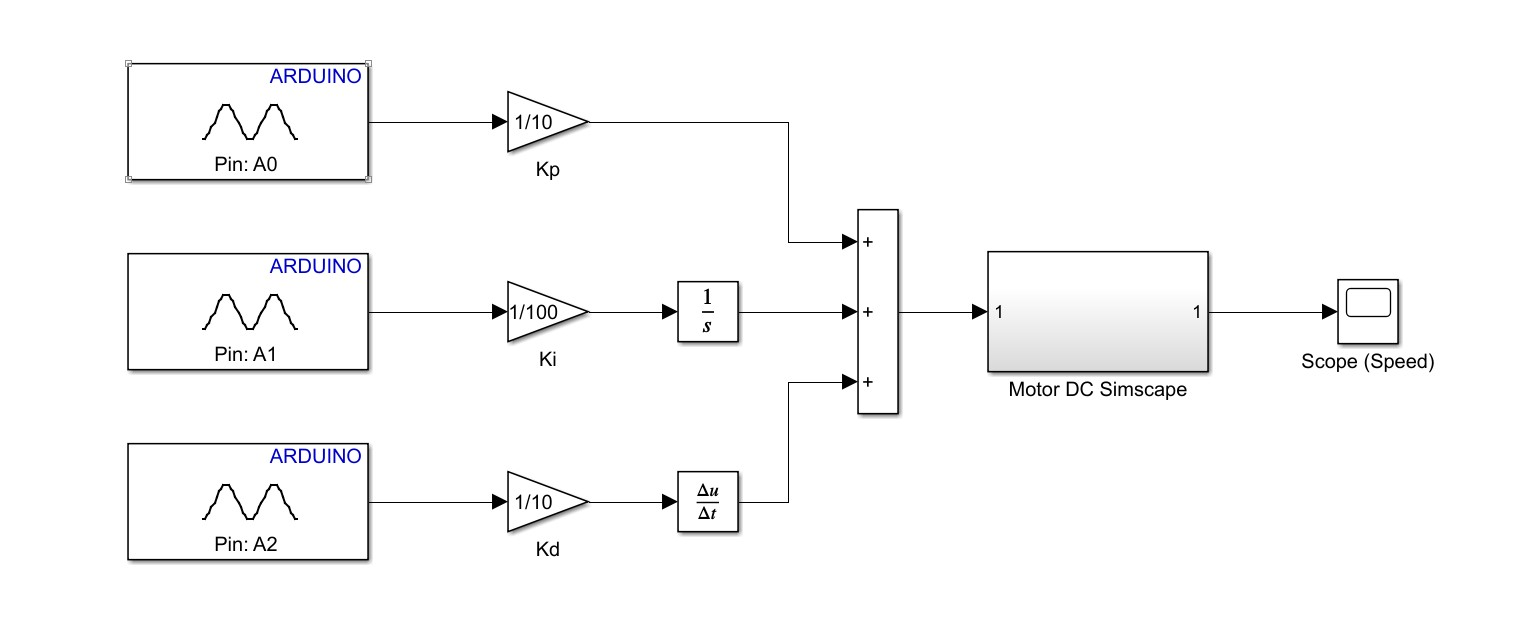
\includegraphics[width=7.5cm]{Gambar Lain/asimscape_pid.jpg}
%		\end{column}%
%		\hfill%
%		\begin{column}{0.48\textwidth}
%			Hasil
%			\color{blue}\rule{\linewidth}{4pt}
%			\begin{center}
%				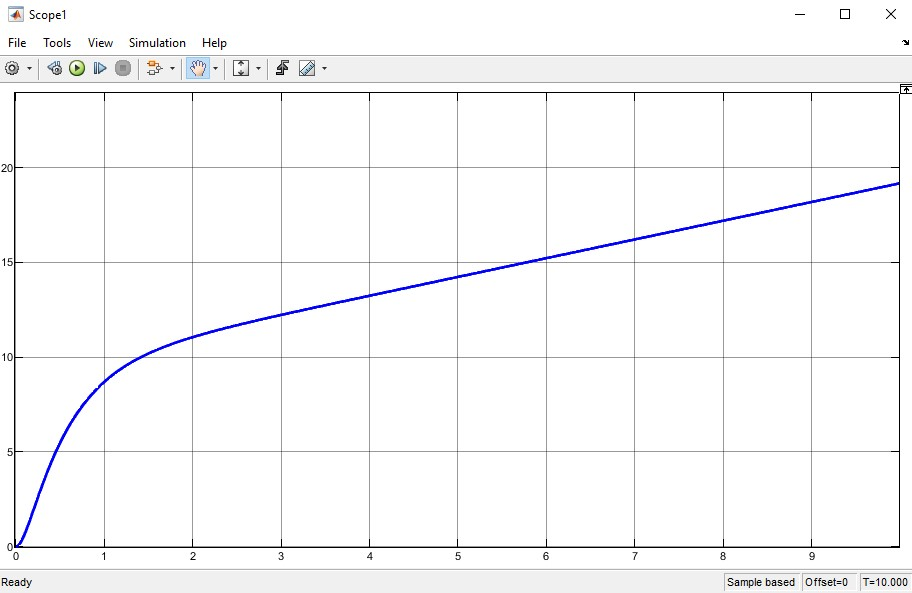
\includegraphics[width=7.5cm]{Gambar Lain/asimscape_pid_scope.jpg}
%			\end{center}
%		\end{column}
%	\end{columns}
%\end{frame}

%\begin{frame}{Tampilan Board Pada Simulasi Arduino-Simulink}
%	\centering
%	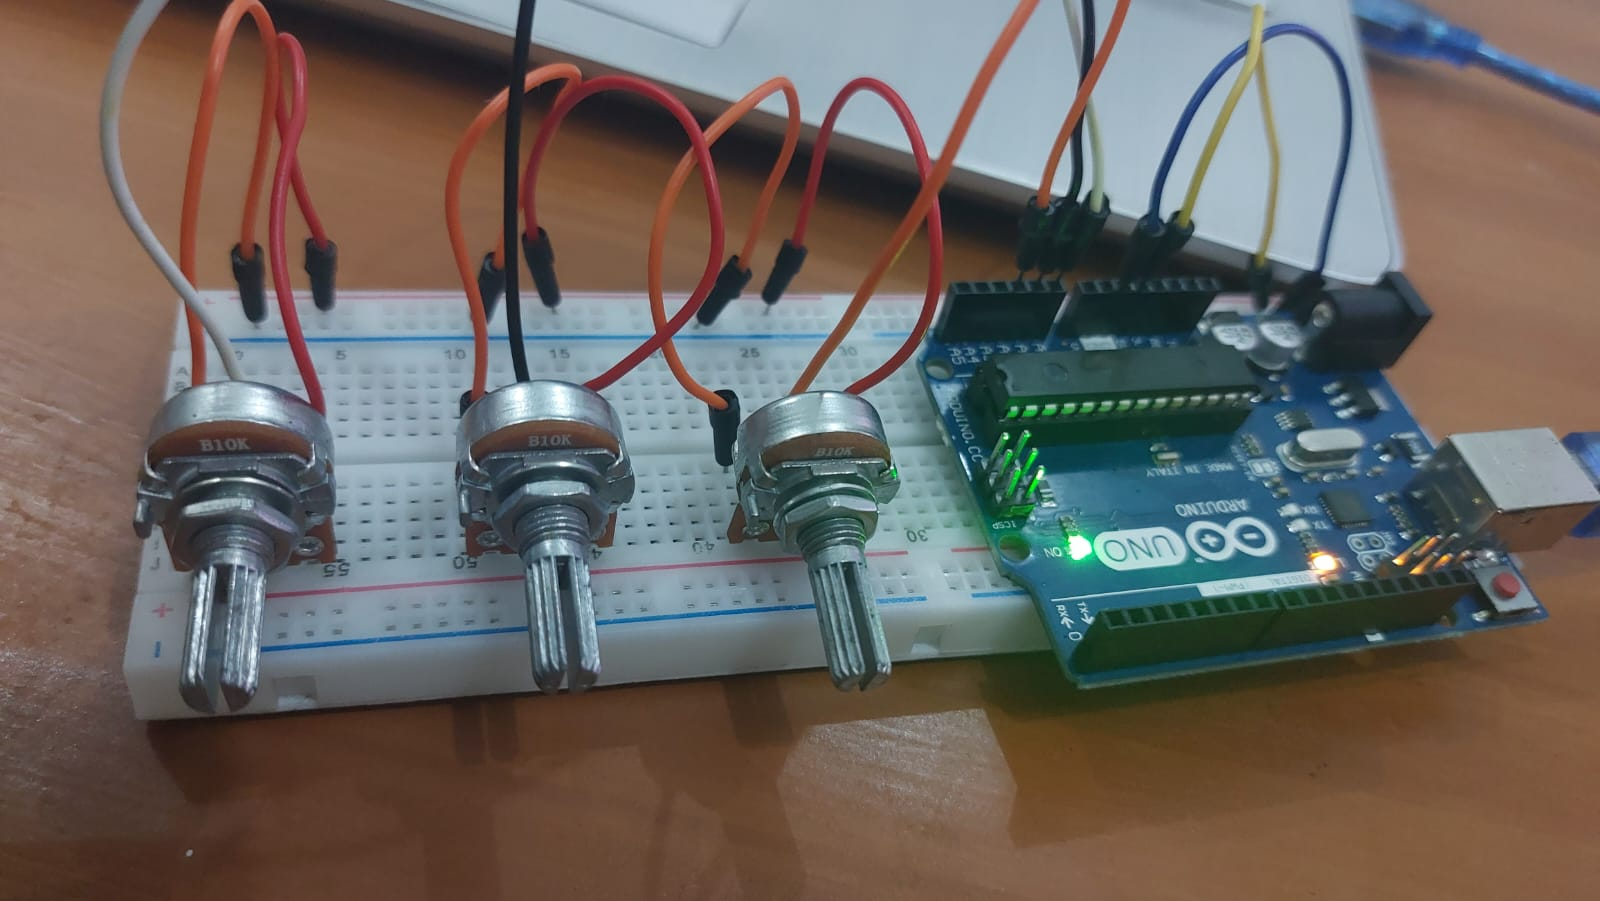
\includegraphics[width=10cm]{Gambar Lain/potentio-arduino.jpeg}
%\end{frame}

%\begin{frame}{Identifikasi Sistem Pada Simulasi Arduino-Simulink}
%	\centering
%	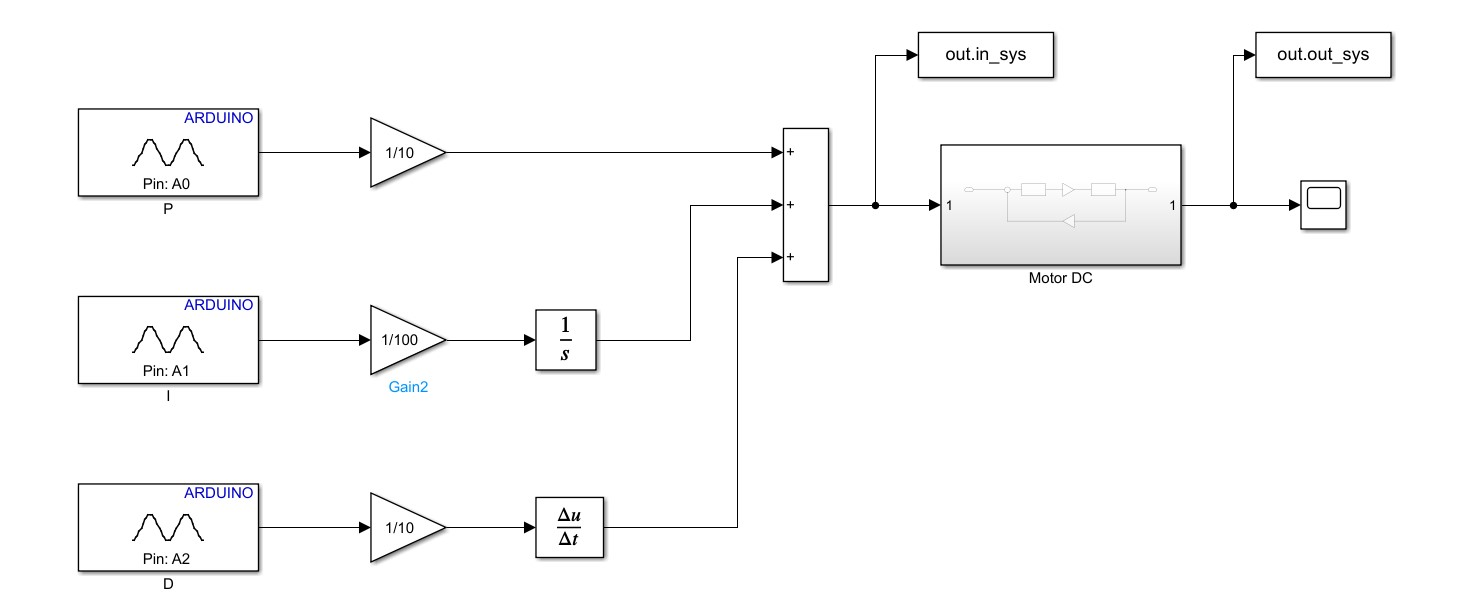
\includegraphics[width=12cm]{Hasil Matlab/blokdiagramident.jpg}
%\end{frame}
%
%\begin{frame}{Proses Identifikasi Sistem}
%	\begin{columns}[T] % align columns
%		\begin{column}{0.48\textwidth}
%			Identifikasi Sistem
%			\color{black}\rule{\linewidth}{4pt}
%			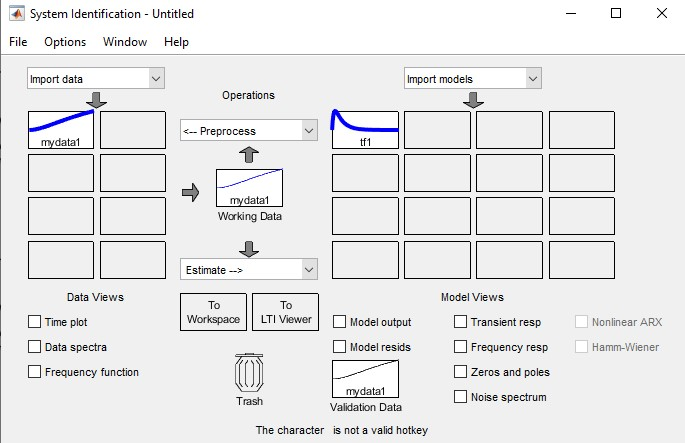
\includegraphics[width=7.5cm]{Hasil Matlab/prosesident.jpg}
%		\end{column}%
%		\hfill%
%		\begin{column}{0.48\textwidth}
%			Hasil Transfer Function
%			\color{blue}\rule{\linewidth}{4pt}
%			\begin{center}
%				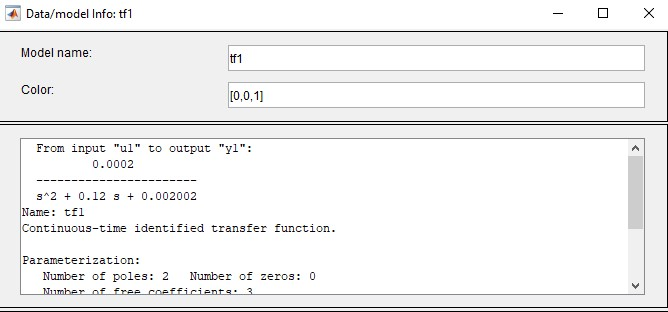
\includegraphics[width=7.5cm]{Hasil Matlab/hasiltf.jpg}
%			\end{center}
%		\end{column}
%	\end{columns}
%\end{frame}

%\begin{frame}{GUI Processing}
%	\centering
%	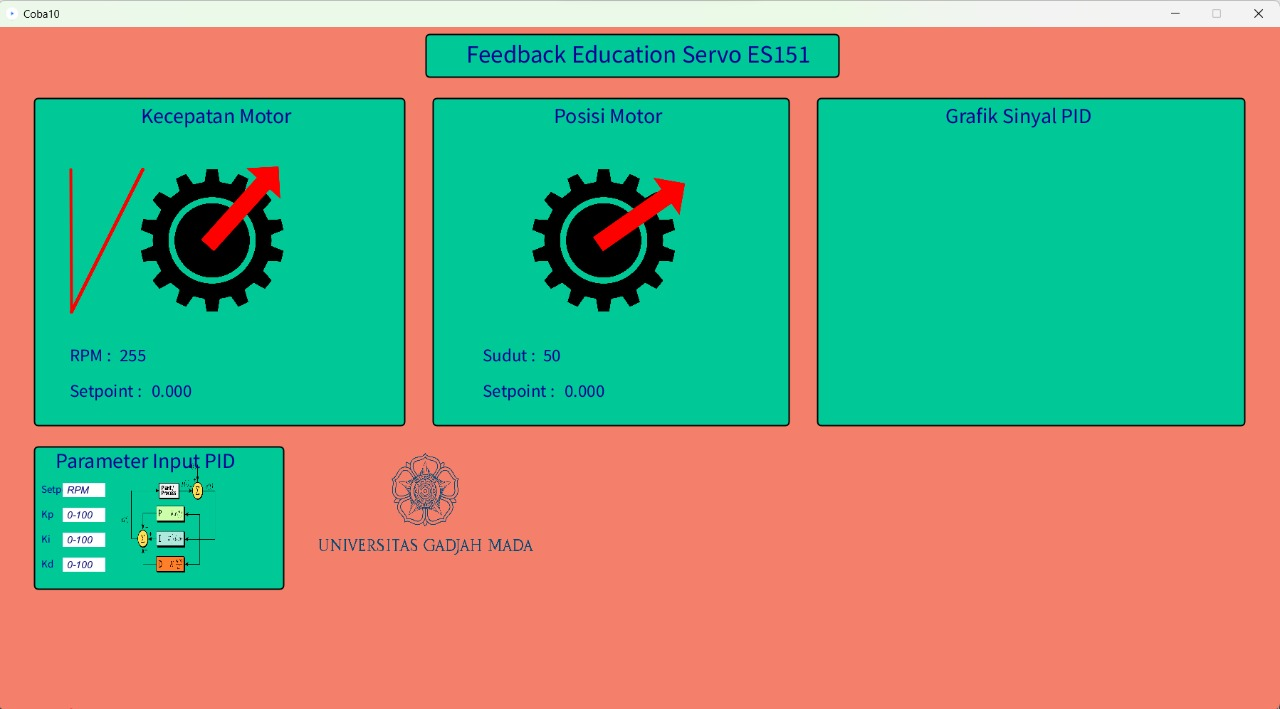
\includegraphics[width=10cm]{Gambar Lain/guiprocessing.jpeg}
%\end{frame}

\end{document}


